\documentclass[12pt]{article}
\usepackage[utf8]{inputenc}
\usepackage{amsmath}
\usepackage{amsfonts}
\usepackage{amssymb}
\usepackage{graphicx}
\usepackage{hyperref}
\usepackage{geometry}
\usepackage{tikz}
\usepackage{pgfplots}
\pgfplotsset{compat=1.18}

\geometry{a4paper, margin=1in}
\usepackage{parskip}
\usepackage{amsthm}
\usepackage{stmaryrd}
\theoremstyle{definition}
\newtheorem{definicion}{Definición}[section]
\newtheorem{ej}{Ejemplo}[section]
\newtheorem{ejercicio}{Ejercicio}[section]

\theoremstyle{plain}
\newtheorem{teo}{Teorema}[section]
\newtheorem{coro}{Corolario}[teo]
\newtheorem{lema}[teo]{Lema}
\newtheorem{prop}{Proposición}[section]
\newtheorem{obs}{Observación}[section]

\usepackage{listings}
\usepackage{amsmath}

\lstset{
    basicstyle=\ttfamily,
    columns=fullflexible,
    mathescape=true
}

\renewcommand{\proofname}{Demostración}

\title{Resumen de Comunicaciones}
\date{\today}

\begin{document}
\newgeometry{top=8cm}

\maketitle

\restoregeometry 

\newpage
\tableofcontents

\newpage
\section{Introducción a las Comunicaciones}

\subsection{Motivación y Conceptos Fundamentales}

En términos primitivos, la comunicación consiste en la transferencia de información entre distintos puntos mediante la variación de una propiedad física (voltaje, corriente, señales electromagnéticas) a través de un medio de transmisión. Con el avance de la tecnología y la democratización de los sistemas digitales, las comunicaciones han evolucionado rápidamente, impulsadas por los gobiernos en contextos de defensa y seguridad, y por la industria en contextos de comercio y entretenimiento. La convergencia de estas motivaciones ha dado lugar a un ecosistema altamente desarrollado.

\begin{definicion}[Red de Computadoras]
Una red de computadoras es un conjunto de computadoras autónomas interconectadas mediante una sola tecnología. Se considera que dos computadoras están interconectadas si tienen la capacidad de intercambiar información. La interconexión física puede realizarse a través de medios guiados (cobre, fibra óptica) o no guiados (enlaces de radio, microondas, satélites).
\end{definicion}

Es indispensable establecer la frontera conceptual entre una red de computadoras y un sistema distribuido.

\begin{obs}[Red de Computadoras vs. Sistema Distribuido]
En un \textbf{sistema distribuido}, un conjunto de computadoras independientes se presenta ante sus usuarios como un único sistema coherente, empleando una capa de software (middleware) que provee cohesión y transparencia. En una \textbf{red de computadoras}, esta coherencia no existe por diseño: las máquinas exponen sus particularidades (hardware y sistema operativo) y los usuarios o aplicaciones deben gestionar explícitamente la comunicación con los equipos remotos. La diferencia fundamental recae en la abstracción provista por el software, no en el hardware subyacente.
\end{obs}

\subsection{Hardware de Red}

Al hablar de hardware de red nos referimos a las cuestiones técnicas implicadas en el diseño e implementación de dichas redes en términos de componentes físicos y su interacción. Existen muchos tipos de redes y muchas variaciones de cada tipo, por lo que encontrar categorías en las cuales caigan absolutamente todas las redes es casi imposible. De este modo nos concentraremos en solamente dos aspectos: la tecnología de transmisión y la escala.

\subsubsection{Tecnología de Transmisión}

Hablando en sentido general, existen dos tipos de tecnología de transmisión que se emplean de forma predominante en la actualidad: los enlaces de difusión (broadcast) y los enlaces de punto a punto.

\begin{itemize}
  \item \textbf{Enlaces de difusión (Broadcast):} 
  En este tipo de redes, todas las máquinas comparten un único canal de comunicación. Los paquetes enviados por una máquina son recibidos por todas las demás máquinas de la red. Cada paquete contiene un campo de dirección que especifica el destinatario. Cuando una máquina recibe un paquete, verifica esta dirección; si el paquete está destinado a ella, lo procesa, de lo contrario, lo ignora. Los sistemas de difusión soportan la transmisión a todos los destinos simultáneamente utilizando un código de dirección especial (operación de broadcast) y, frecuentemente, la transmisión a un subconjunto de máquinas (operación de multicast). Un ejemplo típico de enlace de difusión son las redes inalámbricas.

  \item \textbf{Enlaces de punto a punto:} 
  Conectan pares individuales de máquinas. Para transmitir un paquete desde el origen hasta el destino en una red de punto a punto, el mensaje puede tener que visitar una o más máquinas intermedias. Dado que frecuentemente existen múltiples rutas de diferentes longitudes, los algoritmos de enrutamiento resultan fundamentales en la arquitectura de estas redes. La transmisión de punto a punto con un solo emisor y un solo receptor se denomina unidifusión (unicast).
\end{itemize}

\subsubsection{Escala de la Red}

El segundo criterio fundamental para la clasificación de redes es su escala física, es decir, la distancia que abarca la comunicación. La escala determina las tecnologías de hardware, los medios de transmisión y los protocolos de acceso al medio requeridos. Los sistemas interconectados se clasifican según su distancia en las siguientes categorías principales:

\begin{itemize}
  \item \textbf{Redes de Área Personal (PAN, Personal Area Network):} 
  Permiten la comunicación de dispositivos dentro del rango de acción de una persona, típicamente del orden de 1 metro. El caso de uso habitual es la interconexión de periféricos de computadora o dispositivos portátiles de forma inalámbrica.

  \item \textbf{Redes de Área Local (LAN, Local Area Network):} 
  Redes que operan dentro de un único edificio o campus, abarcando distancias de decenas de metros hasta un kilómetro. Debido a su extensión limitada, el tiempo de transmisión en el peor de los casos es acotado y conocido, lo que permite latencias bajas, bajas tasas de error y altos anchos de banda. Se dividen principalmente en:
  \begin{itemize}
    \item \textbf{Alámbricas:} Dominadas por la tecnología Ethernet (IEEE 802.3), operando generalmente bajo una topología conmutada mediante el uso de switches que vinculan enlaces de punto a punto.
    \item \textbf{Inalámbricas:} Dominadas por el estándar WiFi (IEEE 802.11), donde las máquinas se comunican mediante un medio de difusión hacia un punto de acceso (AP, Access Point).
  \end{itemize}

  \item \textbf{Redes de Área Metropolitana (MAN, Metropolitan Area Network):} 
  Abarcan el área geográfica de una ciudad, del orden de 10 kilómetros. El ejemplo clásico es la red de televisión por cable, la cual fue readaptada para proveer conectividad a Internet de dos vías distribuyendo el espectro.

  \item \textbf{Redes de Área Amplia (WAN, Wide Area Network):} 
  Cubren extensiones geográficas masivas, como un país o continente, en un rango de 100 a 1000 kilómetros. Su diseño introduce una separación arquitectónica estricta entre dos componentes:
  \begin{itemize}
    \item Los \textbf{hosts}: Computadoras dedicadas a ejecutar los programas de aplicación.
    \item La \textbf{subred de comunicación}: Encargada exclusivamente del transporte de mensajes entre hosts. A su vez, está conformada por líneas de transmisión (que mueven los bits, ya sea mediante cobre, fibra o enlaces de radio) y elementos de conmutación (enrutadores o routers, que deciden la línea de salida para cada paquete entrante).
  \end{itemize}
  A diferencia de las LAN, la subred y los hosts de una WAN generalmente pertenecen a entidades distintas, por ejemplo, una empresa administra los hosts y un proveedor de servicios de red (ISP, Internet Service Provider) opera la subred.

  \item \textbf{Interredes (Internetworks):} 
  Una interred se forma cuando se interconectan múltiples redes individuales que pueden utilizar tecnologías subyacentes incompatibles. La interconexión se logra a través de puertas de enlace (gateways). Los routers operan en la capa de red como puertas de enlace para traducir y encaminar los paquetes entre las distintas redes. La Internet global constituye el ejemplo primario de una interred.
\end{itemize}

\begin{obs}[VPNs]
Una red privada virtual (VPN, Virtual Private Network) es un tipo de interred que permite a los usuarios conectarse a una red privada a través de una red pública, como Internet. Esto se logra mediante la creación de un ``túnel'' cifrado que protege la información transmitida. Las VPNs son ampliamente utilizadas para garantizar la seguridad y privacidad de los datos, especialmente en entornos corporativos y para el acceso remoto a redes privadas. En otras palabras, una VPN simula una red privada sobre una infraestructura pública, permitiendo a los usuarios acceder a recursos de la red privada como si estuvieran físicamente presentes en ella.
\end{obs}

\subsection{Software de Red}

Para reducir la complejidad de su diseño, la mayoría de las redes modernas están organizadas de forma altamente estructurada mediante una jerarquía de capas o niveles. Cada capa se construye a partir de la que está debajo de ella. El propósito de cada capa es ofrecer ciertos servicios a las capas superiores, ocultando los detalles relacionados con la implementación de dichos servicios.

\subsubsection{Jerarquías de Protocolos}

La comunicación en red se fundamenta en un modelo de capas en el cual las entidades que conforman la misma capa en diferentes máquinas se denominan pares (peers). Los pares pueden ser procesos de software, dispositivos de hardware o incluso seres humanos. La comunicación no ocurre de forma directa y horizontal entre las capas superiores, sino que los datos y la información de control descienden a través de las capas hasta alcanzar el medio físico.

Entre cada par de capas adyacentes existe una \textbf{interfaz}, la cual define las operaciones y servicios primitivos que la capa inferior pone a disposición de la capa superior. Una interfaz limpia y bien definida permite reemplazar la implementación de una capa sin afectar al resto del sistema, abstrayendo los detalles de la implementación en la capa inferior.

\begin{definicion}[Protocolo]
Un protocolo es un conjunto de reglas y convenciones que rigen el formato, el significado y la sincronización de los paquetes o mensajes intercambiados entre entidades pares para establecer la comunicación dentro de una misma capa.
\end{definicion}

\begin{definicion}[Arquitectura de Red y Pila de Protocolos]
Una arquitectura de red es el conjunto de capas y protocolos subyacentes que definen el funcionamiento de la red. Ni los detalles de implementación ni la especificación interna de las interfaces forman parte de la arquitectura. La lista de los protocolos específicos utilizados por un sistema, con un protocolo por capa, se denomina pila de protocolos.
\end{definicion}

\subsubsection{Aspectos de Diseño para las Capas}

Algunos de los aspectos clave de diseño que ocurren en las redes de computadoras están presentes en las diversas capas. A continuación mencionaremos brevemente los más importantes.

\begin{itemize}
  \item \textbf{Confiabilidad:} La confiabilidad de un servicio se refiere a la capacidad de garantizar la entrega de los datos sin pérdidas, errores o duplicaciones. Esto se logra mediante mecanismos como acuses de recibo (ACKs), retransmisiones, control de flujo, redundancia, etc... Es fundamental sabiendo que las comunicaciones pueden estar sujetas a interferencias, fallos de hardware o congestión en la red (medios imperfectos). Otro aspecto de la confiabilidad consiste en encontrar una ruta funcional a través de la red, lo cual puede implicar el uso de algoritmos de \textbf{enrutamiento}.
  \item \textbf{Direccionamiento y nombramiento:} Dado que existen múltiples computadoras interconectadas, cada capa necesita un mecanismo para identificar unívocamente a los emisores y receptores involucrados en una transmisión específica. Este proceso se conoce como direccionamiento en las capas inferiores y nombramiento en las capas superiores.
  \item \textbf{Control de flujo y asignación de recursos:} Es imperativo contar con mecanismos que eviten que un emisor rápido sature o inunde de datos a un receptor lento, resolviéndose usualmente mediante retroalimentación. Asimismo, la red debe asignar los recursos compartidos (como el ancho de banda) de manera eficiente y gestionar la \textbf{congestión} cuando la cantidad de información a transmitir supera la capacidad del sistema.
  \item \textbf{Escalabilidad y adaptabilidad:} Con esto nos referimos a la capacidad de la red para crecer y adaptarse a un número creciente de usuarios, dispositivos y tráfico sin degradar significativamente el rendimiento, al igual que la posibilidad de mutar y adoptar nuevas tecnologías. Esto implica diseñar protocolos y arquitecturas que puedan manejar eficientemente el aumento de la carga, la expansión geográfica y la evolución de la red.
  \item \textbf{Seguridad:} La seguridad en las comunicaciones de red abarca la protección de los datos y la infraestructura contra accesos no autorizados. Esto incluye la implementación de cifrado, autenticación, control de acceso, detección de intrusiones y políticas de seguridad para garantizar la confidencialidad e integridad de la información transmitida. 
\end{itemize}

Existen otros aspectos de diseño que son importantes en ciertas capas que no hemos mencionado, más no significa que sean menos importantes. Por ejemplo, la eficiencia espectral (maximizar la cantidad de datos transmitidos por unidad de tiempo) es un aspecto crítico en las capas físicas y de enlace de datos, mientras que la latencia y el ancho de banda son consideraciones clave en las capas superiores.

\subsubsection{Tipos de Servicios}

Una capa puede ofrecer a la capa superior dos tipos fundamentales de servicio:

\begin{itemize}
  \item \textbf{Servicio orientado a la conexión:} Modelado a partir del sistema telefónico. El usuario del servicio primero establece una conexión, la utiliza y finalmente la libera. Se comporta como un canal dedicado que generalmente preserva el orden de los datos. Se divide en dos variantes:
  \begin{itemize}
    \item \textbf{Secuencias de mensajes:} Conserva los límites físicos de los mensajes (por ejemplo, dos mensajes de 1024 bytes se reciben como dos unidades distintas).
    \item \textbf{Flujo de bytes:} La conexión es un flujo continuo sin límites en los mensajes (por ejemplo, 2048 bytes recibidos no revelan si fueron enviados juntos o en fragmentos).
  \end{itemize}

  \item \textbf{Servicio sin conexión:} Modelado a partir del sistema postal. Cada mensaje lleva la dirección de destino completa y es enrutado a través de nodos intermedios de forma independiente a los mensajes subsecuentes. Cuando no incluye confirmación de recepción, este modelo se denomina \textbf{servicio de datagramas}.
\end{itemize}

Cada uno de estos servicios puede caracterizarse según su \textbf{confiabilidad}. Un servicio es confiable si garantiza la entrega de los datos sin pérdidas, habitualmente mediante el uso de acuses de recibo (ACKs). La confirmación de recepción introduce sobrecarga y retardo temporal en la red. Aplicaciones como la transferencia de archivos exigen flujos de bytes confiables, mientras que aplicaciones multimedia en tiempo real, como la voz sobre IP (VoIP), toleran la pérdida esporádica de datos pero exigen la mínima latencia que proveen los servicios no confiables (sin confirmación).

\subsubsection{Primitivas de Servicios}

Un servicio se especifica formalmente mediante un conjunto de primitivas disponibles a los procesos de usuario. Estas primitivas indican al servicio que ejecute alguna acción o que informe sobre la acción de una entidad par. En un servicio simple orientado a la conexión. Las primitivas típicas son: \texttt{connect, send, receive, listen, accept, disconnect}. En un servicio sin conexión, las primitivas típicas son: \texttt{send, receive}.

\begin{obs}[Servicios vs. Protocolos]
Un \textbf{servicio} es un conjunto de primitivas que una capa proporciona a la capa que está sobre ella. Define la semántica de la interfaz y estipula qué operaciones están disponibles, pero no cómo se implementan. Por el contrario, un \textbf{protocolo} es un conjunto de reglas que rigen el formato y el significado de los paquetes intercambiados entre entidades pares. Las entidades utilizan los protocolos para implementar las definiciones de los servicios ofrecidos. El servicio y el protocolo son ortogonales, un protocolo puede ser modificado o reemplazado sin alterar el servicio visible para la capa superior.
\end{obs}

\subsection{Modelos de Referencia}

La arquitectura de las redes de computadoras se organiza y estandariza mediante modelos de referencia. Los dos modelos que analizaremos son el modelo OSI y el modelo TCP/IP. Aunque ya casi no se utilizan los protocolos asociados con el modelo OSI, el modelo en sí es bastante general y sigue siendo válido. Asimismo, las características en cada nivel siguen siendo muy importantes. El modelo TCP/IP tiene las propiedades opuestas: el modelo en sí no se utiliza mucho, pero los protocolos son usados ampliamente. Por esta razón veremos ambos elementos con detalle. Además, algunas veces podemos aprender más de los fracasos que de los éxitos.

\subsubsection{El Modelo de Referencia OSI}

El modelo OSI (Open Systems Interconnection), propuesto por la Organización Internacional de Normalización (ISO), consta de siete capas. Su diseño se basa en 5 principios fundamentales:

\begin{enumerate}
  \item Se debe crear una capa en donde se requiera un nivel diferente de abstracción.
  \item Cada capa debe realizar una función bien definida.
  \item La función de cada capa se debe elegir teniendo en cuenta la definición de protocolos estandarizados internacionalmente.
  \item Es necesario elegir los límites de las capas de modo que se minimice el flujo de información a través de las interfaces.
  \item La cantidad de capas debe ser suficiente como para no tener que agrupar funciones distintas en la misma capa. Además, debe ser lo bastante pequeña como para que la arquitectura no se vuelva inmanejable.
\end{enumerate}

Las siete capas del modelo OSI son:

\begin{enumerate}
  \item \textbf{Capa Física:} Encargada de la transmisión de bits puros a través de un canal de comunicación. Define las especificaciones eléctricas, mecánicas y de temporización del medio de transmisión.
  \item \textbf{Capa de Enlace de Datos:} Transforma un medio de transmisión puro en una línea libre de errores para la capa de red. Divide los datos en tramas, administra el acceso al medio y gestiona el control de errores y de flujo. Otra cuestión que surge en la capa de enlace de datos (y en la mayoría de las capas superiores) es cómo evitar que un transmisor rápido inunde de datos a un receptor lento. Tal vez sea necesario algún mecanismo de regulación de tráfico para notificar al transmisor cuando el receptor puede aceptar más datos.
  \item \textbf{Capa de Red:} Controla el funcionamiento de la subred. Su función principal es el enrutamiento de paquetes desde el origen hasta el destino, gestionando la congestión y permitiendo la interconexión de redes heterogéneas. En las redes de difusión, el problema de encaminamiento es simple, por lo que con frecuencia la capa de red es delgada o incluso inexistente.
  \item \textbf{Capa de Transporte:} Acepta los datos de la capa de sesión, los divide en unidades más pequeñas si es necesario y asegura que todos los fragmentos lleguen correctamente al otro extremo. Es la primera capa verdaderamente de extremo a extremo (end-to-end).
  \item \textbf{Capa de Sesión:} La capa de sesión permite a los usuarios en distintas máquinas establecer sesiones entre ellos. Las sesiones ofrecen varios servicios, incluyendo el control del diálogo (llevar el control de quién va a transmitir), el manejo de tokens (evitar que dos partes intenten la misma operación crítica al mismo tiempo) y la sincronización (usar puntos de referencia en las transmisiones extensas para reanudar desde el último punto de referencia en caso de una interrupción).
  \item \textbf{Capa de Presentación:} Se enfoca en la sintaxis y la semántica de la información transmitida, gestionando la representación y codificación abstracta de los datos.
  \item \textbf{Capa de Aplicación:} Contiene los protocolos de alto nivel que los usuarios y las aplicaciones necesitan para la comunicación en red (ej. HTTP, FTP, SMTP).
\end{enumerate}

La siguiente figura ilustra el modelo OSI y sus capas.

\begin{figure}[h]
  \centering
  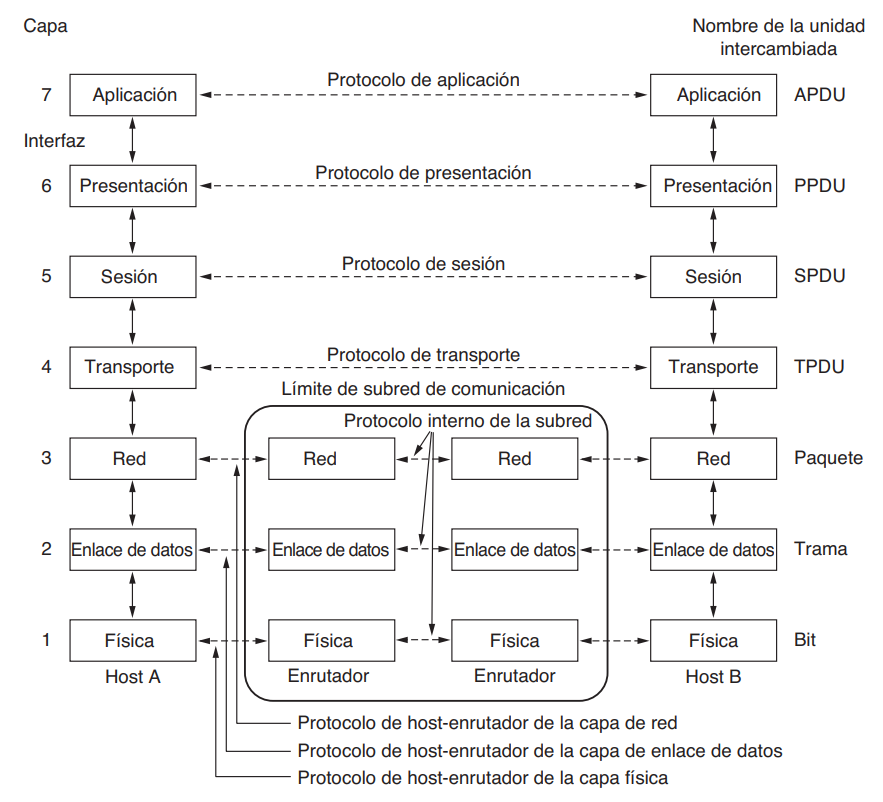
\includegraphics[width=0.90\textwidth]{imgs/1.2.png}
\end{figure}

\subsubsection{El Modelo de Referencia TCP/IP}

El modelo TCP/IP, desarrollado inicialmente por ARPA (Advanced Research Projects Agency) para la red ARPANET, se diseñó con el objetivo principal de conectar múltiples redes de manera transparente y garantizar la supervivencia de la comunicación frente a fallos en el hardware de la subred. El mismo se definió por primera vez en 1974 por Cerf y Kahn. 

Consta de cuatro capas:

\begin{enumerate}
  \item \textbf{Capa de Enlace (Host-to-Network):} Es la capa más baja. En el modelo original no está estrictamente definida como una capa funcional, sino como una interfaz que indica que el host debe conectarse a la red utilizando algún protocolo que le permita enviar paquetes IP.
  \item \textbf{Capa de Interred (Internet):} Eje central de la arquitectura. Su función es inyectar paquetes en cualquier red y que viajen de manera independiente hacia el destino. Incluso pueden llegar en un orden totalmente diferente al orden en que se enviaron, en cuyo caso es responsabilidad de las capas más altas volver a ordenarlos, si se desea una entrega en orden. La capa de interred define un formato de paquete y un protocolo oficial llamado IP (Internet Protocol), además de un protocolo complementario llamado ICMP (Internet Control Message Protocol) que le ayuda a funcionar. La tarea de la capa de interred es entregar los paquetes IP a donde se supone que deben ir. Aquí el ruteo de los paquetes es sin duda el principal aspecto, al igual que la congestión (aunque el IP no ha demostrado ser efectivo para evitar la congestión).
  \item \textbf{Capa de Transporte:} Diseñada para permitir que las entidades pares en los nodos de origen y destino mantengan una conversación de extremo a extremo. Define dos protocolos principales: 
  \begin{itemize}
    \item TCP (Transmission Control Protocol): es un protocolo confiable orientado a la conexión que permite que un flujo de bytes originado en una máquina se entregue sin errores a cualquier otra máquina en la interred. Este protocolo segmenta el flujo de bytes entrante en mensajes discretos y pasa cada uno a la capa de interred. En el destino, el proceso TCP receptor vuelve a ensamblar los mensajes recibidos para formar el flujo de salida. El TCP también maneja el control de flujo para asegurar que un emisor rápido no pueda inundar a un receptor lento con más mensajes de los que pueda manejar.
    \item UDP (User Datagram Protocol): es un protocolo sin conexión, no confiable para aplicaciones que no desean la asignación de secuencia o el control de flujo de TCP y prefieren proveerlos por su cuenta. También se utiliza mucho en las consultas de petición-respuesta de una sola ocasión del tipo cliente-servidor, y en las aplicaciones en las que es más importante una entrega oportuna que una entrega precisa, como en la transmisión de voz o video.
  \end{itemize}
  \item \textbf{Capa de Aplicación:} Contiene los protocolos de alto nivel, fusionando las funcionalidades de las capas de sesión, presentación y aplicación del modelo OSI. Algunos de los más importantes que veremos más adelante: el Sistema de nombres de dominio (DNS), HTTP (el protocolo para recuperar páginas de la World Wide Web), y RTP (el protocolo para transmitir medios en tiempo real, como voz o películas).
\end{enumerate}

\subsubsection{Comparación entre los Modelos OSI y TCP/IP}

\subsection{Evolución y Redes de Ejemplo (TO DO (MUCHO TEXTO))}
\newpage
\section{Capa Física}

Como mencionamos en la sección anterior, la capa física es la encargada de transmitir la información a través del medio físico mediante lo que se conoce como \textbf{señales}.

\subsection{Bases Teóricas para la Comunicación de Datos}

\begin{definicion}[Señal]
  Definimos una \textbf{señal} como la variación de una magnitud física como un voltaje, corriente, onda electromagnética, etc., en función del tiempo. En este contexto, utilizamos las señales para representar la información que queremos transmitir. Si representamos el valor de la magnitud física como una función del tiempo $f(t)$, podemos modelar el comportamiento de la señal y analizarlo matemáticamente.
\end{definicion}

\begin{definicion}[Componentes de una señal]
  Una señal puede caracterizarse por los siguientes componentes:
  \begin{itemize}
    \item Un \textbf{ciclo} de una señal es la porción de la señal que se repite periódicamente. Es decir, es el conjunto de puntos de la función que se repite a lo largo del tiempo.
    \item El \textbf{periodo} mide el tiempo que tarda una onda en completar un ciclo. Se denota como $T$ y se mide en segundos.
    \item La \textbf{frecuencia} de una señal es la cantidad de veces que se repite un ciclo de la señal en un segundo. Se mide en Hertz (Hz) y es el inverso del periodo de la señal, es decir, $f = \frac{1}{T}$, donde $T$ es el periodo. Es importante destacar que hablar de la frecuencia de una señal solo tiene sentido si la misma es periódica.
    \item La \textbf{amplitud} de una señal es la máxima variación de la magnitud física que representa la señal. Se mide en las mismas unidades que la magnitud física, por ejemplo, voltios para un voltaje o amperios para una corriente.
    \item La \textbf{longitud de onda} es la distancia que recorre la señal en un ciclo completo. Se denota como $\lambda$ y se mide en metros. La longitud de onda está relacionada con la frecuencia y la velocidad de propagación de la señal mediante la ecuación $\lambda = \frac{v}{f}$, donde $v$ es la velocidad de propagación de la señal en el medio.
  \end{itemize}
\end{definicion}

\subsubsection{Análisis de Fourier}

A principios del siglo XIX, el matemático francés Jean-Baptiste Fourier demostró que cualquier función periódica de comportamiento razonable, $g(t)$ con un periodo $T$, se puede construir como la suma de un número (posiblemente infinito) de senos y cosenos:

$$g(t) = \frac{a_0}{2} + \sum_{n=1}^{\infty} a_n \sin\left(2\pi nft\right) + b_n \cos\left(2\pi nft\right)$$

donde $f = \frac{1}{T}$ es la frecuencia fundamental, $a_n$ y $b_n$ son las amplitudes de seno y coseno del $n$-ésimo armónico, y $a_0$ es una constante que representa el valor promedio de la función. Esta representación se conoce como \textbf{serie de Fourier}. Podemos reconstruir la función original $g(t)$ a partir de sus componentes de frecuencia, lo que nos permite analizar y manipular señales de manera más efectiva.

Es posible manejar una señal de datos con una duración finita con sólo imaginar que el patrón completo se repite de manera indefinida. 

Podemos calcular los coeficientes de la serie de Fourier mediante las siguientes ecuaciones:
\begin{align}
  a_n &= \frac{2}{T} \int_{0}^{T} g(t) \sin\left(2\pi nft\right) dt \notag \\
  b_n &= \frac{2}{T} \int_{0}^{T} g(t) \cos\left(2\pi nft\right) dt \notag \\
  a_0 &= \frac{2}{T} \int_{0}^{T} g(t) dt \notag
\end{align}

La relevancia de todo esto para la comunicación de datos es que los canales reales afectan a las señales de manera diferente según las frecuencias que componen la señal. Es más, sabemos con certeza que ningún dispositivo puede transmitir señales a través de un medio físico sin perder cierta potencia en el proceso. 

Si todas las frecuencias de una señal se disminuyen de manera uniforme, la señal se atenúa pero no se distorsiona, lo cual sería ideal. Sin embargo, en la práctica, los canales reales no afectan a todas las frecuencias de manera uniforme, lo que puede llevar a la distorsión de la señal y a la pérdida de información. Por lo tanto, es importante diseñar sistemas de comunicación que puedan compensar estas pérdidas y distorsiones para garantizar una transmisión efectiva de la información.

\subsubsection{Señales de Ancho de Banda Limitado}

\begin{definicion}[Ancho de banda]
  El \textbf{ancho de banda} de un canal de comunicación es la diferencia entre la frecuencia más alta y la frecuencia más baja que puede transmitir el canal sin una atenuación considerable de la señal. Se mide en Hertz (Hz) y es un factor crítico en la determinación de la capacidad de transmisión de datos del canal. Un mayor ancho de banda permite transmitir más información en un período de tiempo determinado (aunque vuelve al sistema susceptible a captar mayor cantidad de ruido e interferencias), mientras que un ancho de banda limitado puede restringir la velocidad de transmisión y afectar la calidad de la señal. En otras palabras, el ancho de banda define el rango de frecuencias que un canal puede manejar de manera efectiva.

  Las señales que van desde cero hasta una frecuencia máxima se llaman señales de \textbf{banda base}. Las que se desplazan para ocupar un rango de frecuencias más altas, como es el caso de todas las transmisiones inalámbricas, se llaman señales de \textbf{pasa-banda}.

  Este concepto también se utiliza para filtrar señales, por ejemplo en las comunicaciones de radio, donde se utilizan filtros de paso de banda para permitir que solo ciertas frecuencias pasen a través del canal, mientras que otras son bloqueadas.

  Es estrictamente necesario diferenciar las dos interpretaciones del término en este contexto: el \textbf{ancho de banda analógico} refiere a la propiedad física del medio descrita anteriormente. En contraste, el \textbf{ancho de banda digital} refiere a la tasa máxima de transferencia de datos de un canal, medida en bits por segundo (bps). Un canal con un mayor ancho de banda analógico permite alcanzar un mayor ancho de banda digital, pero el límite exacto de la tasa de transmisión (bps) estará acotado matemáticamente por el ancho de banda en Hz y el nivel de ruido presente en el medio.
\end{definicion}

\subsubsection{La Tasa de Datos Máxima de un Canal}

La capacidad de transmisión de un canal está restringida matemáticamente por su ancho de banda analógico y por la presencia de interferencias en el medio físico. Existen dos teoremas fundamentales en la teoría de la información que establecen el límite superior de la tasa de datos, diferenciando entre canales ideales y canales con ruido.

\begin{teo}[Teorema de Nyquist]
En un canal ideal (libre de ruido) con un ancho de banda finito $B$, la señal filtrada puede reconstruirse por completo tomando exactamente $2B$ muestras por segundo. Si la señal transmitida consta de $V$ niveles discretos, la tasa de datos máxima está dada por:
$$C = 2B \log_2(V)$$
donde $C$ es la capacidad máxima del canal en bits por segundo (bps), $B$ es el ancho de banda en Hertz (Hz) y $V$ es la cantidad de niveles de señal discretos (cantidad de simbolos distintos que se pueden transmitir).
\end{teo}

El teorema de Nyquist demuestra que, en ausencia de ruido, si se pasa una señal cualquiera a través de un filtro pasa-bajas con un ancho de banda $B$, la señal filtrada se puede reconstruir por completo tomando sólo $2B$ muestras por segundo.

\begin{teo}[Teorema de Shannon]
En un canal real sujeto a ruido aleatorio (ruido térmico), la capacidad máxima de transmisión depende de la relación entre la potencia de la señal y la potencia del ruido. La tasa de datos máxima está dada por:
$$C = B \log_2\left(1 + \frac{S}{N}\right)$$
donde $C$ es la capacidad máxima en bits por segundo (bps), $B$ es el ancho de banda en Hertz (Hz), $S$ es la potencia de la señal y $N$ es la potencia del ruido. La relación $\frac{S}{N}$ se conoce como la relación señal a ruido.
\end{teo}

Debido a la gran variación de la relación señal a ruido, en la práctica se expresa en una escala logarítmica utilizando decibeles (dB), mediante la fórmula:
$$\text{SNR}_{\text{dB}} = 10 \log_{10}\left(\frac{S}{N}\right)$$

El teorema de Shannon establece la cota superior teórica para la transferencia de información en cualquier canal sujeto a ruido aleatorio.

\subsection{Medios de Transmisión Guiados}

El propósito de la capa física es transportar bits de una máquina a otra a través de un medio. Los medios de transmisión guiados confinan la señal dentro de un conducto físico y sólido, como el alambre de cobre o la fibra de vidrio.

\subsubsection{Medios Magnéticos}

Una forma de transferir datos consiste en escribirlos en un soporte de almacenamiento magnético u óptico (como cintas de alta densidad o discos físicos) y transportar dicho soporte físicamente a la máquina de destino. 

Este método posee una \textbf{latencia} extremadamente alta (el tiempo de transporte físico se mide en horas o días), pero su \textbf{ancho de banda efectivo} es destacable, pudiendo alcanzar tasas equivalentes a cientos de Gigabits o Terabits por segundo si se transportan grandes volúmenes de datos físicamente de una sola vez.

\subsubsection{Par Trenzado}

El par trenzado es el medio guiado más antiguo y de uso más extendido. Consiste en dos cables de cobre aislados, típicamente de 1 milímetro de grosor, entrelazados en forma helicoidal, de manera análoga a la estructura de una molécula de ADN. 

Dos cables paralelos actúan como una antena. Al trenzarlos, las ondas electromagnéticas emitidas por los cables se cancelan mutuamente, reduciendo la radiación y mejorando significativamente la inmunidad frente al ruido externo. La señal se transmite típicamente como una diferencia de voltaje entre ambos cables. Se pueden tender varios kilómetros de par trenzado sin necesidad de amplificación, pero en distancias mayores la señal se atenúa demasiado y se requieren repetidores. El ancho de banda depende del grosor del cable y de la distancia que recorre, pero en muchos casos se pueden lograr varios megabits/seg durante pocos kilómetros.

Los enlaces de comunicaciones se clasifican según su direccionalidad en tres modos operativos:
\begin{itemize}
    \item \textbf{Simplex:} La transmisión de datos ocurre en una única dirección fija (el flujo es unidireccional).
    \item \textbf{Half-duplex:} La comunicación puede ocurrir en ambas direcciones, pero de forma alternada, es decir, solamente en una dirección a la vez.
    \item \textbf{Full-duplex:} La comunicación puede ocurrir en ambas direcciones de manera simultánea (requiere mecanismos de cancelación de eco o el uso de múltiples pares).
\end{itemize}

\subsubsection{Cable Coaxial}

El cable coaxial ofrece un mayor ancho de banda y un nivel superior de protección contra interferencias electromagnéticas en comparación con el par trenzado. 

Está compuesto por un alambre central de cobre macizo (núcleo), rodeado por un material aislante. Sobre el material aislante se sitúa un conductor exterior cilíndrico (generalmente una malla de cobre trenzado), el cual a su vez está recubierto por una funda protectora de plástico. El conductor exterior trenzado proporciona un blindaje que bloquea el ruido eléctrico externo y evita la fuga de la señal interna. Esta construcción permite transmitir a velocidades superiores y alcanzar distancias mayores que las soportadas por los pares trenzados convencionales.

\subsubsection{Líneas Eléctricas}

Esta tecnología propone la reutilización de la infraestructura de cableado eléctrico existente dentro de un edificio para el transporte de señales de datos. 

La principal dificultad técnica de las líneas eléctricas radica en la presencia de ruido eléctrico severo, generado por la conmutación y operación de electrodomésticos, y en las variaciones de las propiedades eléctricas de las instalaciones. Para que los datos no interfieran con la distribución de energía, las señales digitales deben modularse y transmitirse en bandas de frecuencia completamente separadas de la corriente eléctrica.

\subsubsection{Fibra Óptica}

La fibra óptica transmite información utilizando la luz como portadora. Un sistema de transmisión óptico consta de tres componentes fundamentales: una fuente de luz (diodo emisor de luz o láser), el medio de transmisión (un núcleo de vidrio o sílice fundido ultradelgado) y un detector (un fotodiodo que convierte los fotones entrantes en pulsos eléctricos).

\begin{itemize}
    \item \textbf{Fundamentos ópticos y propagación:} Este sistema de transmisión tendría fugas de luz y sería inútil en la práctica si no fuera por un principio fundamental de la física. Cuando un rayo de luz pasa de un medio a otro con distinto índice de refracción, el rayo se refracta. Sin embargo, si el rayo incide en el límite entre ambos medios a un ángulo mayor que un cierto valor crítico, la luz no se refracta hacia el exterior, sino que se refleja por completo hacia el interior del primer medio. Este fenómeno se conoce como reflexión interna total. En un cable de fibra óptica, el núcleo de vidrio se recubre con un revestimiento que posee un índice de refracción menor. Esta configuración confina la luz en el interior del núcleo, causando que los rayos reboten en las paredes internas y se propaguen a lo largo del cable sin pérdida de información hacia el exterior.
    
    \item \textbf{Monomodo y Multimodo:}
    \begin{itemize}
        \item \textbf{Multimodo:} Dado que cualquier rayo que incida por encima del ángulo crítico se reflejará internamente, muchos rayos diferentes pueden rebotar en múltiples ángulos (modos) de manera simultánea. Debido a la dispersión modal (los distintos rayos recorren distancias diferentes y llegan al receptor en momentos distintos, ensanchando el pulso original), se restringe su uso a distancias cortas.
        \item \textbf{Monomodo:} Si el diámetro del núcleo se reduce al orden de unas pocas longitudes de onda de la luz, el cable actúa como una guía de ondas. La luz se propaga en línea recta como un rayo único sin rebotar. Emplea láseres de alta precisión, evita por completo la dispersión modal y es el estándar absoluto para enlaces de larga distancia.
    \end{itemize}
    
    \item \textbf{Métodos de empalme:} La conexión entre dos fibras requiere precisión óptica rigurosa. Existen tres métodos:
    \begin{itemize}
        \item \textbf{Conectores:} Se utilizan conectores mecánicos para unir los extremos, facilitando la conexión en paneles, pero introduciendo una pérdida de señal del 10 al 20 por ciento.
        \item \textbf{Empalmes mecánicos:} Alineación rigurosa de los extremos perfectamente cortados de las fibras dentro de un tubo especial. Presentan una pérdida aproximada del 10 por ciento.
        \item \textbf{Fusión:} Consiste en fundir y unir los extremos de las fibras mediante un arco eléctrico. Forma una unión sólida y continua que casi no presenta atenuación en la señal transmitida.
    \end{itemize}
\end{itemize}

\subsection{Transmisión Inalámbrica}

En contraposición a los medios guiados, la transmisión inalámbrica utiliza el espacio libre para la propagación de ondas electromagnéticas.

\subsubsection{El Espectro Electromagnético y Bandas ISM}

Cuando los electrones se mueven, crean ondas electromagnéticas que se pueden propagar por el espacio (incluso en el vacío). La transmisión inalámbrica se basa en la modulación de ondas electromagnéticas. Al conectar una antena del tamaño apropiado a un circuito eléctrico, las ondas electromagnéticas se pueden difundir de manera eficiente y un receptor las puede captar a cierta distancia. Toda la comunicación inalámbrica se basa en este principio. 

En el vacío, todas las ondas electromagnéticas viajan a la misma velocidad sin importar cuál sea su frecuencia. Esta velocidad se conoce como velocidad de la luz, $c \approx 3 \times 10^8$ m/s. La relación entre la velocidad de propagación, la frecuencia y la longitud de onda está dada por la ecuación $c = f \lambda$, donde $f$ es la frecuencia y $\lambda$ es la longitud de onda.

En la siguiente figura se muestra el espectro electromagnético. Las porciones de radio, microondas, infrarrojo y luz visible del espectro se pueden utilizar para transmitir información mediante la modulación de la amplitud, frecuencia o fase de las ondas. La luz ultravioleta, los rayos X y los rayos gamma serían todavía mejores, debido a sus frecuencias más altas, pero son difíciles de producir y de modular, no se propagan bien entre edificios y son peligrosos para los seres vivos. Las bandas que se listan en la parte inferior de la figura son los nombres oficiales de la ITU (Unión Internacional de Telecomunicaciones) y se basan en las longitudes de onda, por lo que la banda LF va de 1 a 10 km (aproximadamente de 30 a 300 kHz). Los términos LF, MF y HF se refieren a las frecuencias baja, media y alta, respectivamente. Está claro que al asignar los nombres nadie esperaba rebasar los 10 MHz, por lo que las bandas más altas se denominaron después como bandas de muy, ultra, súper, extrema y tremendamente alta frecuencia. \textbf{Más allá de eso ya no hay nombres, pero podrían sonar bien las designaciones de increíble, asombrosa y prodigiosamente alta frecuencia (IHF, AHF y PHF).}

\begin{obs}
  Con \textbf{espectro} nos referimos a la representación de la intensidad (amplitud o potencia) de una señal en función de la frecuencia. En otras palabras, el espectro de una señal es una función en el dominio de la frecuencia e indica qué frecuencias están presentes en la señal y con qué fuerza.
\end{obs}

Los rangos de frecuencia más relevantes utilizados en las telecomunicaciones se clasifican de la siguiente manera:

\begin{itemize}
    \item \textbf{Ondas de radio:} Son omnidireccionales (viajan en todas las direcciones) y fáciles de generar. Sus propiedades de propagación son altamente dependientes de la frecuencia. A bajas frecuencias atraviesan obstáculos con facilidad y siguen la curvatura de la Tierra, experimentando una atenuación por pérdida de trayectoria. A frecuencias superiores, viajan en línea recta, rebotan en obstáculos y se refractan en la ionosfera, lo que permite comunicaciones de mayor alcance.
    
    \item \textbf{Microondas:} Operan por encima de los 100 MHz. Viajan en línea recta, lo que permite enfocar la energía en un haz estrecho mediante antenas parabólicas, incrementando significativamente la relación señal a ruido. Sus principales vulnerabilidades son el desvanecimiento por multitrayectorias (causado por refracción atmosférica) y, en frecuencias cercanas o superiores a los 4 GHz, la atenuación severa por absorción de agua (lluvia).
    
    \item \textbf{Infrarrojo:} Ondas no guiadas de corto alcance altamente direccionales. Su característica limitante y definitoria es la incapacidad de atravesar objetos sólidos. Esta restricción física representa una ventaja en el diseño de redes, ya que aísla los sistemas en recintos adyacentes evitando interferencias y elevando la seguridad frente al espionaje.
    
    \item \textbf{Ondas de luz:} Comunicación óptica de espacio libre (típicamente empleando láseres). Ofrece anchos de banda sumamente elevados a bajo costo y sin requerimientos de licenciamiento. Es estrictamente unidireccional y exige una alineación extremadamente precisa. Sus desventajas principales incluyen la dispersión térmica (interferencia por corrientes de convección en el aire) y la atenuación ante condiciones meteorológicas adversas como lluvia o niebla.
\end{itemize}

Dado que el espectro radioeléctrico es un recurso físico finito y susceptible a interferencias cruzadas, su uso se encuentra fuertemente regulado. Sin embargo, existen bandas de frecuencia exentas de licencia, denominadas \textbf{bandas ISM} (Industrial, Científica y Médica), tales como 900 MHz, 2.4 GHz y 5.8 GHz. Cualquier dispositivo puede transmitir en estas bandas, condicionado a restricciones estrictas de potencia máxima y, frecuentemente, a la implementación de técnicas de dispersión de señal para minimizar la interferencia.

\subsubsection{Satélites de Comunicación}

En su forma más simple, podemos considerar un satélite de comunicaciones como un enorme repetidor de microondas en el cielo que contiene varios transpondedores, cada uno de los cuales escucha en cierta porción del espectro, amplifica la señal entrante y después la retransmite en otra
frecuencia para evitar interferencia con la señal entrante. Este modo de operación se llama tubo doblado. Se puede agregar un procesamiento digital para manipular o redirigir por separado los flujos de datos en toda la banda, o el satélite puede recibir información digital y retransmitirla. Esta forma de regeneración de señales mejora el desempeño si se le compara con un tubo doblado, ya que el satélite no amplifica el ruido en la señal que va hacia arriba. Los haces que descienden pueden ser amplios y cubrir una fracción considerable de la superficie de la Tierra, o pueden ser estrechos y cubrir un área de unos cuantos cientos de kilómetros de diámetro.

Nos centraremos en los \textbf{satélites geoestacionarios}, que se encuentran a una altitud de aproximadamente 36.000 km sobre el ecuador. A esta altura, la velocidad angular del satélite coincide con la de rotación de la Tierra, por lo que el satélite parece estar fijo en el cielo desde cualquier punto de la superficie terrestre. Esto permite que las antenas receptoras permanezcan apuntando hacia el mismo lugar sin necesidad de seguimiento. Sin embargo, la distancia considerable introduce un retardo de propagación significativo (aproximadamente 250 ms) y una atenuación notable de la señal. Además, la cobertura de un satélite geoestacionario es limitada a aproximadamente un tercio de la superficie terrestre.

Una propiedad importante de los satélites es que son medios de difusión por naturaleza. Cuesta lo mismo enviar un mensaje a miles de estaciones dentro de la huella de un transpondedor que enviarlo a una sola. Para algunas aplicaciones esta propiedad es muy útil. Por ejemplo, podríamos imaginar un satélite difundiendo páginas web populares a las cachés de una gran cantidad de computadoras dispersas sobre un área amplia. Aun cuando podemos simular la difusión mediante líneas de punto a punto, es probable que la difusión vía satélite sea más económica. Por otro lado, desde el punto de vista de la privacidad, los satélites son un completo desastre: todos pueden escucharlo todo. Es esencial el cifrado cuando se requiere seguridad.

\subsection{Modulación Digital y Multiplexación}

La transmisión de información requiere codificar bits digitales en señales físicas que el medio pueda transportar (modulación) y, frecuentemente, compartir la capacidad total de un mismo canal entre múltiples comunicaciones simultáneas (multiplexación).

\subsubsection{Transmisión en Banda Base}

La transmisión en banda base consiste en la conversión directa de un flujo de datos digitales en variaciones de voltaje o luz que se envían por el medio, ocupando las frecuencias desde cero hasta un límite dado. Para realizar esta conversión se utilizan \textbf{códigos de línea}. Algunos de los códigos de línea más importantes son:

\begin{itemize}
  \item \textbf{NRZ (No Retorno a Cero):} Es la codificación más simple, donde un nivel de voltaje positivo representa un 1 y un voltaje negativo representa un 0. Su principal deficiencia es la falta de recuperación de reloj: una larga secuencia de ceros o unos consecutivos provoca que el receptor a la larga pierda la sincronización y no pueda determinar dónde termina un bit y comienza el siguiente, resultando en errores de interpretación de la señal.
  \item \textbf{NRZI (No Retorno a Cero Invertido):} Es una variante de NRZ que resuelve parcialmente el problema de sincronización. En este esquema, un 1 se representa mediante una transición de voltaje (de alto a bajo o de bajo a alto), mientras que un 0 se representa por la ausencia de transición. Esto garantiza al menos una transición por cada bit 1, pero aún puede haber largas secuencias de ceros consecutivos que provoquen pérdida de sincronización.
  \item \textbf{Codificación Manchester:} Resuelve el problema de sincronización forzando una transición de voltaje en la mitad de cada periodo de bit (de alto a bajo para un 1, y de bajo a alto para un 0). Esta transición funciona como una señal de reloj incorporada. Su desventaja fundamental es que requiere el doble de ancho de banda analógico que NRZ para transmitir la misma tasa de datos.
  \item \textbf{Codificación bipolar:} Utiliza tres niveles de voltaje: positivo, negativo y cero. Un 1 se representa alternando entre los niveles positivo y negativo, mientras que un 0 se representa con el nivel cero. Esto permite la detección de errores mediante la verificación de la alternancia de los niveles de voltaje.
\end{itemize}

A la hora de elegir diseñar la codificación en una transmisión, es fundamental considerar los siguientes aspectos:

\begin{itemize}
  \item \textbf{Eficiencia del ancho de banda:} \\
  Con NRZ, la señal puede alternar entre los niveles positivo y negativo hasta cada 2 bits (en caso de alternar 1s y 0s). Esto significa que necesitamos un ancho de banda de por lo menos $B/2$ Hz cuando la tasa de bits es de $B$ bits/seg. Esta relación proviene de la tasa de Nyquist, por lo tanto no podemos operar el esquema NRZ a una mayor velocidad sin usar más ancho de banda. Por lo general el ancho de banda es un recurso limitado. Entre más altas sean las frecuencias de las señales su atenuación es cada vez mayor, lo que las hace menos útiles, además las señales de frecuencias más altas también requieren componentes electrónicos más rápidos.

  Una estrategia para utilizar el ancho de banda limitado con más eficiencia es usar más de dos niveles de señalización. Por ejemplo, si utilizamos cuatro voltajes podemos enviar 2 bits a la vez como un solo símbolo. Este diseño funcionará siempre y cuando la señal en el receptor sea lo bastante fuerte como para diferenciar los cuatro niveles. La tasa a la que cambia la señal es entonces la mitad de la tasa de bits, por lo que se reduce el ancho de banda necesario. La tasa a la que cambia la señal se denomina \textbf{tasa de símbolo} para diferenciarla de la \textbf{tasa de bits}. La tasa de bits es la tasa de símbolo multiplicada por el número de bits por símbolo.

  \item \textbf{Recuperación de reloj:} \\
  En todos los esquemas que codifican bits en símbolos, el receptor debe saber cuándo termina un símbolo y empieza el siguiente para decodificar los bits de forma correcta. Como ya mencionamos, en la codificación NRZ, largas secuencias de ceros o unos consecutivos pueden provocar que el receptor pierda la sincronización y no pueda determinar dónde termina un bit y comienza el siguiente.

  Los relojes exactos serían útiles para resolver este problema, pero son una solución costosa para un equipo básico. Recordando que vamos a sincronizar bits en enlaces que operan a muchos megabits/seg, por lo que el reloj tendría que variar menos de una fracción de un microsegundo durante la sucesión más larga permitida. Esto podría ser razonable para los enlaces lentos o mensajes cortos, pero no es una solución general.

  Una estrategia es enviar una señal de reloj separada al receptor. Otra línea de reloj no representa mucho para los buses de computadora o los cables cortos en donde hay muchas líneas en paralelo, pero sería un desperdicio para la mayoría de los enlaces de red, ya que si tuviéramos otra línea para enviar una señal, la podríamos usar para enviar datos.

  Para resolver este problema, se utiliza la codificación Manchester, descrita anteriormente. Como ya vimos, esto introduce un nuevo problema: la codificación Manchester requiere el doble de ancho de banda que NRZ para transmitir la misma tasa de bits.
\end{itemize}





\subsubsection{Transmisión Pasa-Banda}

La transmisión pasa-banda regula una onda analógica continua, denominada \textbf{onda portadora}, para transportar la señal digital. Al alterar características de la portadora, la señal se desplaza a un rango de frecuencias superior predeterminado.

\begin{itemize}
    \item \textbf{Técnicas de modulación básicas:} 
    \begin{itemize}
        \item[b)] \textbf{ASK (Modulación por Desplazamiento de Amplitud):} Dos o más niveles de amplitud representan los datos.
        \item[c)] \textbf{FSK (Modulación por Desplazamiento de Frecuencia):} Se utilizan dos o más frecuencias diferentes.
        \item[d)] \textbf{PSK (Modulación por Desplazamiento de Fase):} La fase de la onda portadora se desplaza sistemáticamente en intervalos fijos.
    \end{itemize}
    \begin{figure}[h]
      \centering
      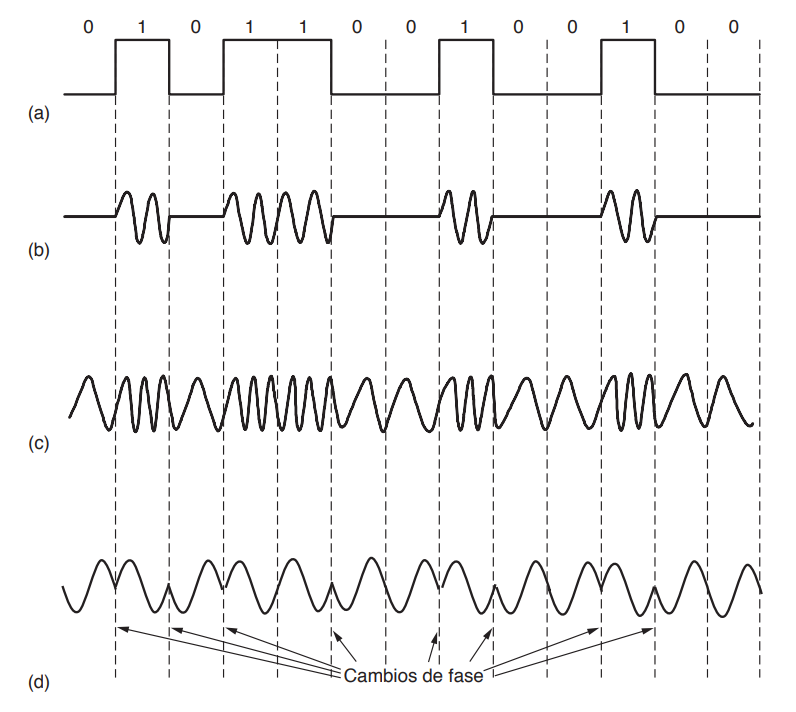
\includegraphics[width=0.7\textwidth]{imgs/2.1.png}
    \end{figure}
\end{itemize}

También tenemos técnicas de modulación más avanzadas, como la \textbf{QAM (Modulación de Amplitud en Cuadratura)} que combina ASK y PSK para transmitir múltiples bits por cada cambio de señal. Los esquemas QAM (como QAM-16 o QAM-64) se representan mediante \textbf{diagramas de constelación}, donde cada punto en el plano representa un estado específico de amplitud y fase, denominado \textbf{símbolo}.

\subsubsection{Multiplexación}

En las comunicaciones resulta muy interesante en terminos de eficiencia utilizar canales de transmisión compartidos por múltiples usuarios. Este estilo de canales, requiere la implementación de técnicas de \textbf{multiplexación}. Para lograr que las señales no se mezclen ni se corrompan entre sí, el canal debe dividirse lógicamente. Las dos dimensiones principales para realizar esta división son la frecuencia y el tiempo.

\begin{itemize}
  \item \textbf{Multiplexación por División de Frecuencia (FDM):}\\
  Aprovecha la transmisión pasa-banda para compartir un canal físico en el dominio de la frecuencia. De manera intuitiva, funciona igual que las emisoras de radio comerciales: todas las estaciones transmiten al mismo tiempo a través del mismo aire, pero cada una sintoniza una frecuencia diferente para que los receptores puedan separarlas.
  \begin{itemize}
    \item \textbf{FDM clásico:} El ancho de banda analógico total del medio se divide en múltiples bandas de frecuencia separadas, asignando cada banda a un usuario o flujo de datos distinto de forma continua. Para evitar que las señales se solapen e interfieran entre canales adyacentes, se introducen pequeños rangos de frecuencia inactivos denominados \textbf{bandas de guarda}.
    \item \textbf{OFDM (FDM Ortogonal):} Una versión más avanzada donde el espectro se divide en un gran número de subportadoras estrechas. A diferencia del FDM tradicional, en OFDM las bandas de las subportadoras se superponen para ahorrar espacio, pero se diseñan matemáticamente ortogonales entre sí para no interferir. Esto elimina la necesidad de bandas de guarda y mejora drásticamente la eficiencia espectral.
  \end{itemize}

  \item \textbf{Multiplexación por División de Tiempo (TDM):}\\
  TDM es una alternativa a FDM. Aquí, los usuarios toman turnos para transmitir. Cada usuario utiliza la totalidad del ancho de banda del canal, pero únicamente durante fracciones de tiempo periódicas denominadas \textbf{ranuras de tiempo}. Se pueden agregar pequeños intervalos de \textbf{tiempo de guarda}, los cuales son análogos a una banda de guarda de frecuencia, para tener en cuenta las pequeñas variaciones de sincronización.
\end{itemize}


\newpage
\section{Capa de Enlace: Subcapa de Control de Enlace Lógico (LLC)}

La capa de enlace consiste en los algoritmos y protocolos que permiten la comunicación confiable y eficiente de unidades completas de información llamadas \textbf{tramas} (frames) entre dos máquinas adyacentes. Por adyacente, queremos decir que las dos máquinas están conectadas mediante un canal de comunicaciones en el cual los bits se entregan en el mismo orden en que fueron enviados.

En esta sección, nos centraremos en la subcapa de control de enlace lógico, que es la parte de la capa de enlace que se encarga de proporcionar un servicio confiable a la capa de red. A diferencia de la subcapa de control de acceso al medio (MAC), LLC es independiente al hardware.

\subsection{Cuestiones de Diseño de la Capa de Enlace}

La capa de enlace de datos utiliza los servicios de la capa física para enviar y recibir bits a través de los canales de comunicación. Tiene varias funciones específicas, entre las que se incluyen:

\begin{itemize}
  \item Proporcionar a la capa de red una interfaz de servicio bien definida.

  \item Manejar los errores de transmisión.

  \item Regular el flujo de datos para que los emisores rápidos no saturen a los receptores lentos.
\end{itemize}

Para cumplir con estas metas, la capa de enlace de datos toma los paquetes que obtiene de la capa de red y los encapsula en tramas para transmitirlos. Cada trama contiene un encabezado, un campo de carga útil (payload) para almacenar el paquete y un terminador. El manejo de las
tramas es la tarea más importante de la capa de enlace de datos.

\subsubsection{Servicios Proporcionados a la Capa de Red}

La capa de enlace de datos puede diseñarse para ofrecer varios servicios. Los servicios reales ofrecidos varían de un protocolo a otro. Tres posibilidades razonables que normalmente se proporcionan son:

\begin{itemize}
  \item \textbf{Servicio sin conexión ni confirmación de recepción:} La capa de enlace de datos simplemente acepta los paquetes de la capa de red, los encapsula en tramas y los envía. No se proporciona ninguna confirmación de recepción. Ethernet es un buen ejemplo de una capa de enlace de datos que provee esta clase de servicio. Esta clase de servicio es apropiada cuando la tasa de error es muy baja, de modo que la recuperación se deja a las capas superiores. También es apropiada para el tráfico en tiempo real, como el de voz, en donde es peor tener retraso en los datos que errores en ellos.
  \item \textbf{Servicio sin conexión con confirmación de recepción:} La capa de enlace acepta los paquetes de la capa de red y los envía. Luego espera una confirmación de recepción. Si no se recibe la confirmación, la trama se puede retransmitir. 802.11 (WiFi) es un buen ejemplo de esta clase de servicio.
  \item \textbf{Servicio con conexión y confirmación de recepción:} La capa de enlace establece una conexión con el otro extremo antes de enviar los paquetes. Este servicio garantiza que cada trama se reciba correctamente y en el orden correcto. 
\end{itemize}

\subsubsection{Entramado}

Para proporcionar el servicio a la capa de red, la capa de enlace de datos debe utilizar el flujo de bits continuo que le entrega la capa física. Dado que la capa física no ofrece garantías de integridad ni mecanismos de delimitación, la capa de enlace debe fragmentar el flujo de bits en tramas, de modo que el receptor pueda identificar inequívocamente el inicio y el fin de cada una. Este proceso se denomina \textbf{entramado}.

Veremos cuatro métodos para llevar a cabo el entramado:

\begin{itemize}
  \item \textbf{Conteo de bytes:} 
  Emplea un campo en el encabezado de la trama para especificar el número de bytes que contiene la misma. Cuando el receptor procesa el encabezado, utiliza este valor para determinar en qué punto exacto finaliza la trama actual. Su deficiencia fundamental es la fragilidad ante errores de transmisión: si el campo de conteo se corrompe por ruido, el receptor perderá la sincronización, ya que leerá el conteo erróneo, procesará el final de la trama en el lugar equivocado y será incapaz de identificar el inicio lógico de las tramas subsiguientes.

  \item \textbf{Bytes bandera con relleno de bytes:} 
  Resuelve el problema de la pérdida de sincronización delimitando el inicio y el fin de cada trama con un byte especial reservado, denominado byte bandera (\texttt{FLAG}). El problema surge cuando el patrón de bits que representa al byte bandera aparece dentro de los datos. Para evitar que el receptor interprete este dato como el final de la trama, el transmisor inserta un byte especial de escape (\texttt{ESC}) justo antes de la aparición del byte bandera en los datos. Este proceso de inyección se conoce como relleno de bytes. Si el propio byte de escape forma parte de los datos útiles, el transmisor lo precede con otro byte de escape. El hardware receptor elimina sistemáticamente estos bytes de escape añadidos antes de entregar el paquete a la capa de red.

  \item \textbf{Bits bandera con relleno de bits:} 
  A diferencia del relleno de bytes, esta técnica permite tramas formadas por cantidades arbitrarias de bits y no exige que los caracteres se definan de a porciones de 8 bits. Cada trama empieza y termina con un patrón de bits específico, convencionalmente \texttt{01111110} (\texttt{0x7E}). Para evitar la interpretación errónea en los datos, se emplea el relleno de bits a nivel de hardware: cada vez que el transmisor encuentra cinco bits \texttt{1} consecutivos en los datos, inserta un bit \texttt{0} forzado en el flujo transmitido. En el extremo receptor, al detectar cinco bits \texttt{1} consecutivos seguidos de un \texttt{0}, este último se descarta automáticamente. Si se detectan seis bits \texttt{1} consecutivos, el receptor sabe que es una bandera delimitadora válida y no parte de los datos.

  \item \textbf{Violaciones de codificación de la capa física:} 
  Este método es aplicable únicamente en redes donde la codificación física a nivel de señal incluye cierta redundancia. Por ejemplo, en la codificación Manchester, cada bit se transmite como dos estados lógicos separados (alto-bajo o bajo-alto). Las combinaciones alto-alto y bajo-bajo son estados ilegales. La capa de enlace puede generar deliberadamente estas violaciones de codificación de la capa física para delimitar el inicio y el fin de las tramas, dado que es imposible que estos patrones aparezcan dentro del flujo de bits codificado válidamente.
\end{itemize}

Muchos protocolos de enlace de datos usan una combinación de estos métodos por seguridad. Un patrón común utilizado para Ethernet y 802.11 es hacer que una trama inicie con un patrón bien definido, conocido como \textbf{preámbulo}. Este patrón podría ser bastante largo (es común que cuente con 72 bits para 802.11) de modo que el receptor se pueda preparar para un paquete entrante. El preámbulo va seguido de un campo de longitud (cuenta) en el encabezado, que se utiliza para localizar el final de la trama.

\subsubsection{Control de Errores}

Una vez resuelto el problema de delimitar las tramas, debemos garantizar que todas ellas se entreguen a la capa de red del destino en el orden correcto. Dado que los canales físicos son inherentemente imperfectos, es necesario implementar mecanismos para lidiar con las tramas que se dañan o se pierden por completo durante la transmisión. La estrategia fundamental consiste en proporcionar al emisor una retroalimentación explícita: el receptor devuelve tramas de control especiales que contienen un \textbf{acuse de recibo} positivo o negativo.

Sin embargo, la retroalimentación por sí sola es insuficiente ante la pérdida absoluta de una trama de datos o de su respectivo acuse de recibo, escenario que dejaría al emisor en un estado de espera infinita. Para evitar este bloqueo lógico, se introducen los \textbf{temporizadores}. Al transmitir una trama, el emisor inicia un reloj configurado con un intervalo de tiempo suficiente para que la trama llegue, sea procesada y regrese la confirmación. Si el temporizador expira sin que haya llegado una respuesta, el emisor asume que ocurrió un fallo y retransmite la trama. 

Esta técnica de retransmisión basada en tiempos límite resuelve el problema del estancamiento, pero introduce una nueva vulnerabilidad: la entrega de tramas duplicadas si el elemento perdido fue únicamente el acuse de recibo. Para resolver esta ambigüedad, el protocolo exige asignar \textbf{números de secuencia} a cada trama saliente, lo que permite al receptor distinguir inequívocamente entre una trama nueva y una retransmisión redundante.

\subsubsection{Control de Flujo}

Un problema crítico de diseño en la capa de enlace de datos (y en las capas superiores) es la discrepancia de capacidades entre un emisor rápido y un receptor lento. Cuando un dispositivo de alto rendimiento transmite tramas de manera sistemática a una velocidad superior a la que el nodo de destino puede procesar, los búferes de recepción se saturan. En consecuencia, el receptor se ve forzado a descartar tramas por falta de espacio, incluso si la transmisión física a través del canal estuvo completamente libre de errores. 

Para evitar esta pérdida de información, los protocolos implementan mecanismos que regulan la transmisión, divididos en dos enfoques principales. El primero es el \textbf{control de flujo basado en retroalimentación}, donde el receptor devuelve información explícita al emisor para autorizarle el envío de más datos o notificarle su estado. El segundo es el \textbf{control de flujo basado en tasa}, un mecanismo integrado en el protocolo que limita la velocidad máxima a la que el emisor puede inyectar datos en el canal, sin requerir notificaciones por parte del receptor.

\subsection{Ejemplo de Protocolo de Enlace de Datos (PPP)}

SONET es el protocolo de capa física que se utiliza con más frecuencia sobre los enlaces de fibra óptica de área amplia que constituyen la espina dorsal de las redes de comunicaciones. Provee un flujo de bits que opera a una tasa de transmisión bien definida, organizado en forma de cargas
útiles de bytes de tamaño fijo. 

Para transportar paquetes sobre SONET, la capa de enlace de datos necesita un mecanismo de entramado específico. El protocolo estándar de Internet utilizado casi universalmente en enrutadores para esta tarea es el \textbf{PPP (Protocolo Punto a Punto)}. Se utiliza para manejar la configuración de detección de errores en los enlaces, soporta múltiples protocolos, permite la autentificación y tiene muchas otras funciones. Con un amplio conjunto de opciones, PPP provee tres características principales:

\begin{itemize}
  \item Un método de entramado estricto orientado a bytes, que delinea sin ambigüedades el final de una trama y el inicio de la siguiente (utilizando banderas especiales y relleno de bytes). El formato también maneja la detección de errores.
  \item Un \textbf{Protocolo de Control de Enlace} (LCP, Link Control Protocol), encargado de activar líneas, probarlas, negociar opciones y desactivarlas en forma ordenada cuando ya no son necesarias.
  \item Un mecanismo para negociar opciones de capa de red con independencia del protocolo de red que se vaya a utilizar. El método elegido debe tener un NCP (Network Control Protocol) distinto para cada capa de red soportada.
\end{itemize}

\subsubsection{Formato de Trama de PPP}

La transmisión de paquetes IP sobre SONET utilizando PPP  casi siempre opera en ``modo no numerado'', proveyendo un servicio sin conexión ni confirmación de recepción, asumiendo que la fibra óptica es un medio sumamente confiable y delegando el manejo de pérdidas a la capa de transporte.

El formato de la trama es el siguiente:
\begin{itemize}
    \item \textbf{Bandera (1 byte):} Todas las tramas PPP comienzan y terminan con el byte estándar \texttt{01111110} (0x7E). PPP emplea relleno de bytes usando un byte de escape (\texttt{01111101} o 0x7D) si la bandera aparece accidentalmente dentro de los datos útiles.
    \item \textbf{Dirección (1 byte):} Se establece a un valor constante (\texttt{11111111}) indicando difusión (todas las estaciones deben aceptar la trama). En un enlace punto a punto real, este campo pierde sentido algorítmico, ya que el único destino posible es el otro extremo de la línea.
    \item \textbf{Control (1 byte):} Se fija en \texttt{00000011}, valor que denota que la trama es del tipo no numerada (sin control estricto de secuencia).
    \item \textbf{Protocolo (1 o 2 bytes):} Identifica qué tipo de datos transporta el campo de carga útil. Permite diferenciar si el contenido es un paquete IPv4, un paquete IPv6, o si se trata de mensajes de control internos del propio enlace (paquetes de LCP o NCP).
    \item \textbf{Carga útil (Variable):} Contiene la información a transmitir. El tamaño máximo se negocia previamente mediante LCP (usualmente 1500 bytes por defecto).
    \item \textbf{Suma de verificación (2 o 4 bytes):} Un código de comprobación de errores estandarizado (CRC, Cyclic Redundancy Check). Si el receptor calcula un CRC distinto al recibido, asume corrupción y descarta la trama sin emitir confirmación ni pedir retransmisión.
\end{itemize}

Cuando PPP se implementa físicamente sobre SONET, se aplica una técnica de aleatorización a los datos antes de la transmisión. Esto garantiza un número elevado de transiciones de voltaje (evitando largas secuencias de ceros o unos) necesarias para mantener la sincronización física del reloj del sistema SONET, mitigando así deficiencias que no puede manejar el simple entramado.



\newpage
\section{Capa de Enlace: Subcapa de Control de Acceso al Medio (MAC)}

En los canales de difusión generalmente se tiene el problema de que varios usuarios pueden intentar transmitir al mismo tiempo, lo que genera colisiones. Para resolver este problema, se utilizan protocolos de acceso al medio (MAC) que determinan cómo los usuarios comparten el canal. 

La subcapa MAC tiene especial importancia en las LAN, en especial las inalámbricas puesto que el canal inalámbrico es de difusión por naturaleza. Debido a que los canales multiacceso y las LAN están muy relacionados, en esta sección analizaremos las LAN en general.

\subsection{El Problema de Asignación del Canal}

El tema central de esta subcapa es la forma de asignar un solo canal de difusión entre usuarios competidores. El canal podría ser una parte del espectro inalámbrico en una región geográfica, o una fibra óptica en donde se conectan varios nodos. Esto no es importante. En ambos casos, el canal conecta a cada usuario con todos los demás, cualquier usuario que utilice todo el canal interfiere con los demás
que también desean usarlo.

\subsubsection{Asignación Estática del Canal}

La asignación estática consiste en dividir la capacidad total de un único canal de comunicación entre $N$ usuarios competidores, asignando a cada uno una fracción fija y exclusiva del recurso. Esta división se implementa convencionalmente mediante las técnicas de multiplexación que vimos anteriormente, como FDM o TDM. Este esquema resulta eficiente únicamente cuando existe una cantidad pequeña, fija y conocida de usuarios que mantienen una carga de tráfico pesada y constante (por ejemplo, transmisiones de radio FM).

Sin embargo, la asignación estática es ineficiente para las redes de computadoras, donde la naturaleza del tráfico de datos opera en ráfagas de alta intensidad. Bajo este esquema, surgen dos deficiencias críticas:

\begin{itemize}
  \item Si un usuario se encuentra inactivo, su porción de ancho de banda (o ranura de tiempo) se pierde por completo, ya que la división estricta prohíbe que otros emisores la utilicen. En consecuencia, la mayor parte del canal permanece ocioso la mayor parte del tiempo.
  \item Si la cantidad de usuarios que desean transmitir supera el límite físico de particiones $N$, el sistema negará el acceso a los emisores excedentes por falta de espectro asignable, incluso si existen canales de otros usuarios temporalmente inactivos.
\end{itemize}

\subsubsection{Supuestos para la Asignación Dinámica de Canales}

Todo el trabajo hecho en esta área se basa en cinco supuestos clave, que se describen a continuación:

\begin{enumerate}
    \item \textbf{Tráfico independiente:} El modelo consta de $N$ estaciones independientes, cada una generando tramas de forma impredecible pero a una tasa de llegada promedio constante (distribución de Poisson). Tras generar una trama, la estación se bloquea lógicamente y detiene su generación hasta que dicha trama logre transmitirse con éxito.
    \item \textbf{Canal único:} La totalidad de las comunicaciones ocurre sobre un único medio físico compartido. Todas las estaciones transmiten y reciben sobre él.
    \item \textbf{Colisiones observables:} Si dos tramas se transmiten en forma simultánea, se traslapan en el tiempo y la señal resultante se altera. Este evento se llama \textbf{colisión}. Todas las estaciones pueden detectar una colisión que haya ocurrido. Una trama en colisión se debe volver a transmitir después. No hay otros errores, excepto aquéllos generados por las colisiones.
    \item \textbf{Tiempo continuo o ranurado:} Se puede asumir que el tiempo es continuo, en cuyo caso la transmisión de una trama puede comenzar en cualquier momento. Por el contrario, el tiempo se puede ranurar o dividir en intervalos discretos (llamados ranuras). En este caso las transmisiones de las tramas deben empezar al inicio de una ranura. Una ranura puede contener 0, 1 o más tramas, correspondientes a una ranura inactiva, una transmisión exitosa o una colisión, respectivamente. 
    \item \textbf{Detección de portadora o sin detección:} Con el supuesto de detección de portadora, las estaciones pueden saber si el canal está en uso antes de intentar usarlo. Si se detecta que el canal está ocupado, ninguna estación intentará utilizarlo. Si no hay detección de portadora, las estaciones no pueden detectar el canal antes de intentar usarlo. Simplemente transmiten. Sólo después pueden determinar si la transmisión tuvo éxito.
\end{enumerate}

\subsection{Protocolos de Acceso Múltiple}

\subsubsection{ALOHA}

ALOHA fue el primer protocolo MAC diseñado para un medio de difusión compartido (originalmente redes de radio). Analizaremos las dos variantes de este protocolo:

\begin{itemize}
    \item \textbf{ALOHA Puro:} La idea básica es sencilla: cuando una estación tiene una trama para enviar, la transmite inmediatamente al canal. No verifica si el medio está ocupado antes de transmitir. 
    
    Dado que las estaciones transmiten en instantes completamente aleatorios, es inevitable que los tiempos de transmisión de dos o más tramas se superpongan. En ALOHA puro, si esto ocurre, decimos que las tramas colisionan y se corrompen mutuamente. La estación central al recibir una trama transmite a todas las estaciones la misma, por lo tanto, si una estación no recibe la trama que envió, sabe que ocurrió una colisión y que su trama se perdió.
    
    Si la trama fue destruida, el emisor simplemente espera un tiempo aleatorio y la envía de nuevo. El tiempo de espera debe ser aleatorio o las mismas tramas chocarán una y otra vez, en sincronía. Los sistemas en los cuales varios usuarios comparten un canal común de modo tal que puede dar pie a conflictos se conocen como sistemas de \textbf{contención}.

    Lo malo de esto es que no importa que tanto se solapen las tramas, con que al menos un bit se superponga, la trama se pierde.
    
    \item \textbf{ALOHA Ranurado:} Para mejorar el ineficiente rendimiento del ALOHA puro, se introdujo una restricción temporal. En ALOHA ranurado, el tiempo continuo se divide en intervalos discretos (ranuras) de tamaño igual al tiempo de transmisión de una trama estándar.
    
    La nueva regla de operación exige que las estaciones estén sincronizadas: cuando una estación genera una trama, no puede transmitirla inmediatamente. Debe esperar obligatoriamente al inicio de la siguiente ranura de tiempo. Para lograr esto, se utiliza una estación especial que transmite una señal al comienzo de cada intervalo.
    
    Esta discreción temporal altera drásticamente la probabilidad de colisiones. Al obligar a que todas las transmisiones comiencen exactamente en el mismo instante, se elimina la posibilidad de solapamientos parciales. Las tramas o colisionan por completo (si dos o más estaciones transmiten en la misma ranura), o no colisionan en absoluto. Al reducir el periodo de vulnerabilidad exactamente a la mitad en comparación con el modelo puro, ALOHA ranurado duplica la eficiencia máxima teórica.
\end{itemize}


\subsubsection{Protocolos de Acceso Múltiple con Detección de Portadora}

La ineficiencia de los sistemas ALOHA radica en que las estaciones no conocen el estado del canal. En muchas redes (particularmente las redes LAN alámbricas), es posible que las estaciones escuchen el canal antes de actuar, mecanismo que se denomina \textbf{detección de portadora}. Los protocolos que utilizan esta característica adaptan su comportamiento para evitar colisiones obvias, mejorando el rendimiento del canal. 

La familia de protocolos \textbf{CSMA} (Carrier Sense Multiple Access) implementan esta idea mediante sus distintas variantes:

\begin{itemize}
    \item \textbf{CSMA persistente-1:} Cuando una estación tiene datos por enviar, escucha el canal. Si está inactivo, transmite inmediatamente. Si está ocupado, la estación se queda escuchando continuamente hasta que el canal se libere, en ese preciso instante, transmite su trama (con probabilidad de 1, de ahí el nombre). Esto evita colisiones con una transmisión en curso, pero si dos o más estaciones están esperando a que termine una transmisión, ambas intentarán transmitir exactamente al mismo tiempo cuando el canal se libere.

    \item \textbf{CSMA no persistente:} Busca solucionar el problema del CSMA persistente-1 siendo menos egoísta. Si una estación desea transmitir y encuentra el canal ocupado, en lugar de quedarse esperando a que finalice la transmisión actual, espera un periodo de tiempo aleatorio y recién entonces vuelve a escuchar el canal. Esto reduce las colisiones, pero introduce retraso.

    \item \textbf{CSMA persistente-p:} Diseñado para canales de tiempo ranurado. Si la estación encuentra el canal inactivo, transmite con una probabilidad $p$. Si no lo hace (con probabilidad $q = 1-p$), espera a la siguiente ranura temporal. Si en esa ranura el canal sigue libre, vuelve a aplicar la lógica anterior. Si el canal está ocupado, espera un tiempo aleatorio e inicia el proceso nuevamente. Es la base conceptual de las redes Wi-Fi (IEEE 802.11).
\end{itemize}

\textbf{CSMA con detección de colisiones}

CSMA evita colisiones al inicio, pero si dos estaciones detectan el canal libre y transmiten simultáneamente, sus señales de todas formas chocarán. En los esquemas anteriores, las estaciones terminan de transmitir toda su trama a pesar de que ya está corrupta, desperdiciando ancho de banda. 

CSMA/CD mejora este comportamiento añadiendo \textbf{detección de colisiones}. Mientras una estación está transmitiendo, el hardware escucha analógicamente la línea. Si la señal que lee es distinta a la que está enviando, sabe inmediatamente que ha ocurrido una colisión. En ese instante, la estación deja de transmitir.

Un aspecto vital en CSMA/CD es que la detección de una colisión no es instantánea debido al retardo de propagación de la señal. Si el tiempo que tarda una señal en viajar de un extremo al otro de la red es $\tau$, en el peor de los casos una estación que inició una transmisión tardará hasta $2\tau$ (el tiempo de viaje de ida y vuelta) en enterarse de que colisionó. Por lo tanto, una estación solo puede estar segura de que tomó el canal (y que nadie más transmitirá) tras haber transmitido durante un tiempo $2\tau$ sin detectar conflictos.

Este protocolo es la base de la clásica LAN Ethernet.

\subsubsection{Protocolos Libres de Colisiones}

Aunque CSMA/CD mejora drásticamente el rendimiento frente al modelo ALOHA, las colisiones siguen ocurriendo durante el periodo de contención, lo cual degrada el desempeño cuando la red tiene una carga alta. Los protocolos libres de colisiones resuelven la contención de manera que el solapamiento de tramas sea imposible por diseño.

\begin{itemize}
    \item \textbf{Protocolo de mapa de bits:} El periodo de contención se divide en $N$ ranuras de tiempo estandarizadas, una para cada estación. Si la estación $j$ desea transmitir, emite un bit de valor 1 durante su ranura respectiva. Al finalizar el periodo de las $N$ ranuras, todas las estaciones saben de forma determinista quién desea transmitir. Las estaciones interesadas transmiten sus tramas en estricto orden numérico secuencial. Evita colisiones absolutas a costa de la sobrecarga obligatoria de transmitir el mapa de bits completo antes de cada ronda de datos.
    
    En la siguiente figura se muestra un ejemplo de mapa de bits con 8 estaciones.
    \begin{figure}[h]
        \centering
        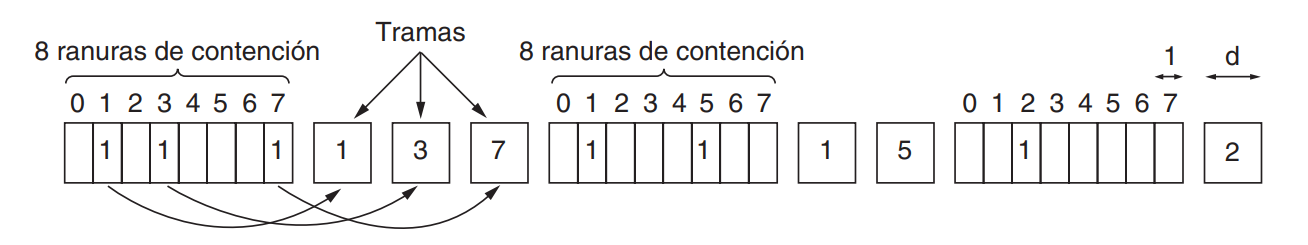
\includegraphics[width=0.8\textwidth]{imgs/4.2.png}
    \end{figure}
    \item \textbf{Paso de token:} Utiliza un mensaje de control lógico especial denominado token. Las estaciones se organizan (física o lógicamente) en una topología de anillo. El token circula sistemáticamente de una estación a otra. Únicamente la estación en posesión del token está autorizada a transmitir datos sobre el canal. Al finalizar, pasa el token.
    \item \textbf{Conteo descendente binario:} Cada estación posee una dirección binaria única de longitud fija. Las estaciones que desean transmitir difunden su dirección bit por bit sincronizadamente, empezando por el bit más significativo. Las direcciones se combinan en el canal mediante una función OR booleana. Si una estación transmite un 0 pero lee un 1 del canal, comprende que compite contra una estación con una dirección mayor, en ese instante se rinde y abandona la contención. La estación con la dirección numérica más alta siempre gana el acceso al medio sin colisionar datos. Este protocolo asume de manera implícita que los retardos de transmisión son insignificantes, de manera que todas las estaciones ven los bits instantáneamente.
\end{itemize}

\subsubsection{Protocolos de Contención Limitada}

Los protocolos de contención pura (como CSMA) ofrecen un buen rendimiento frente a cargas ligeras, pero son deficientes bajo carga alta por el aumento de colisiones. Inversamente, los protocolos libres de colisiones garantizan eficiencia bajo carga saturada, pero generan retrasos innecesarios a carga baja.

Los protocolos de contención limitada buscan combinar las ventajas de ambos, decidiendo dinámicamente qué estaciones pueden competir por el canal según la carga de tráfico.

El \textbf{protocolo de recorrido de árbol adaptable} modela a las estaciones como las hojas de un árbol binario. En la primera ranura posterior a una transmisión exitosa, todas las estaciones (el nodo raíz) intentan transmitir. Si ocurre una colisión, en la siguiente ranura solo las estaciones en la mitad izquierda del árbol (las estaciones bajo ese subárbol) podrán competir. Si vuelve a colisionar, se restringe a la mitad izquierda de esa mitad. Cuando un grupo logra transmitir con éxito o dejar el canal inactivo, el algoritmo cede el turno a la mitad derecha del nivel correspondiente. Este mecanismo ajusta la carga de la contención dinámicamente según el nivel de tráfico.


\subsubsection{Protocolos de LAN Inalámbrica}

Los protocolos CSMA tradicionales fueron diseñados para redes alámbricas, asumiendo que todas las estaciones pueden escucharse entre sí. En los entornos inalámbricos de radio, la potencia de la señal decae rápidamente con la distancia. Esta limitación física invalida los supuestos alámbricos e introduce dos anomalías estructurales que degradan el rendimiento:

\begin{itemize}
    \item \textbf{El problema de la terminal oculta:} Supongamos que la estación $A$ está transmitiendo hacia $B$. Una estación $C$, también desea transmitir a $B$. La estación $C$ escucha el canal antes de transmitir, pero dado que $A$ está fuera de su rango de radio, $C$ no detecta portadora. $C$ concluye erróneamente que el medio está inactivo e inicia su transmisión hacia $B$. Ambas señales colisionan en el receptor $B$, destruyendo la información.

    \item \textbf{El problema de la terminal expuesta:} Supongamos que $B$ está transmitiendo hacia $A$. La estación $C$, que es vecina de $B$, desea iniciar una transmisión hacia una estación lejana $D$. $C$ escucha el canal, detecta la transmisión en curso de $B$, asume que el medio está ocupado y pospone su envío. Sin embargo, este aplazamiento es innecesario y desperdicia ancho de banda: la transmisión de $C$ hacia $D$ no interferiría en absoluto con la recepción que $A$ está haciendo de $B$, porque $A$ está fuera del rango de $C$.
\end{itemize}

Para resolver estas deficiencias, surge el protocolo \textbf{MACA (Multiple Access with Collision Avoidance)}. El concepto en que se basa es que el emisor estimule al receptor para que envíe una trama corta, de manera que las estaciones cercanas puedan detectar esta transmisión y
eviten ellas mismas hacerlo durante la siguiente trama de dato (grande). Se utiliza esta técnica en vez de la detección de portadora.

El proceso de transmisión de datos mediante MACA consiste en:

\begin{enumerate}
    \item Antes de enviar datos, el emisor transmite una trama de control muy corta denominada \textbf{RTS} (Request To Send), indicando explícitamente la longitud de la trama de datos que desea enviar.
    \item Si el receptor está inactivo y recibe el RTS, responde emitiendo una trama \textbf{CTS} (Clear To Send), copiando en ella la longitud anunciada de los datos.
    \item Al recibir el CTS, el emisor inicia inmediatamente la transmisión de los datos reales.
\end{enumerate}

Este mecanismo de intercambio protege el canal controlando a las estaciones vecinas de la siguiente manera:
\begin{itemize}
    \item Resolución de la terminal oculta: Cualquier estación (como $C$ en el primer ejemplo) que escuche el CTS sabe que una estación cercana está a punto de recibir datos. Por lo tanto, extrae la longitud de los datos de la trama CTS y permanece obligatoriamente en silencio durante ese lapso de tiempo.
    \item Resolución de la terminal expuesta: Si una estación escucha un RTS pero no escucha un CTS (como $C$ en el segundo ejemplo), deduce algebraicamente que está cerca del emisor pero lejos del receptor objetivo. En consecuencia, sabe que puede transmitir libremente sin causar colisiones en el destino de esa transmisión, optimizando la concurrencia espacial de la red.
\end{itemize}

Cabe destacar que las propias tramas RTS aún pueden colisionar (si dos estaciones inician el protocolo hacia el mismo destino simultáneamente). Ante esta colisión, el emisor no recibirá el CTS esperado, por lo que abortará el intento, aplicará un tiempo de espera aleatorio y reintentará más tarde.

\subsection{Ethernet}

Ethernet es el estándar dominante en redes de área local (LAN) alámbricas. Existen dos tipos de Ethernet: Ethernet clásica, que resuelve el problema de acceso múltiple mediante el uso de las técnicas que hemos estudiado en esta sección; el segundo tipo es la Ethernet conmutada, en donde los dispositivos llamados switches se utilizan para conectar distintas computadoras. Es importante mencionar que, aunque se hace referencia a ambas como Ethernet, son muy diferentes. La Ethernet clásica es la forma original que operaba a tasas de transmisión de 3 a 10 Mbps. La Ethernet conmutada es en lo que se convirtió la Ethernet y opera a 100, 1000 y 10000 Mbps. Actualmente, en la práctica sólo se utiliza Ethernet conmutada.

A nivel físico, la Ethernet clásica utiliza un cable coaxial grueso o delgado, mientras que la Ethernet conmutada utiliza cables de par trenzado o fibra óptica. Se tendía un cable a lo largo de un edificio y se conectaban las computadoras a este cable mediante un conector. La Ethernet conmutada utiliza un dispositivo mediador llamado switch, que tiene varios puertos, cada uno de los cuales se conecta a una computadora mediante un cable de par trenzado o fibra óptica.


\subsubsection{Formato de la Trama y Restricciones Físicas}

La subcapa MAC de Ethernet encapsula los paquetes de la capa de red en tramas con la siguiente estructura básica:

\begin{itemize}
    \item \textbf{Preámbulo:} Secuencia de 8 bytes (alternando unos y ceros, finalizando en 11) utilizada para la sincronización de reloj en el hardware receptor.
    \item \textbf{Direcciones MAC:} Dos campos de 6 bytes que identifican unívocamente la dirección física de destino y de origen.
    \item \textbf{Tipo/Longitud (2 bytes):} Indica el protocolo de capa de red encapsulado (ej. IPv4, ARP) o, en implementaciones antiguas, la longitud de la carga útil.
    \item \textbf{Datos:} Carga útil proveniente de la capa superior. Está acotada a un máximo estricto de 1500 bytes.
    \item \textbf{Relleno:} Bytes inactivos añadidos si la carga útil es insuficiente para que la trama alcance el tamaño mínimo requerido.
    \item \textbf{Suma de verificación (4 bytes):} Un código CRC-32 (Cyclic Redundancy Check) evaluado por el hardware receptor para detectar corrupciones de bits.
\end{itemize}

\textbf{Límite mínimo de trama:} Para que el mecanismo CSMA/CD detecte colisiones algorítmicamente, la transmisión debe durar al menos el tiempo de propagación de ida y vuelta de la red ($2\tau$). Esto garantiza que el emisor siga transmitiendo (y pueda sensar la colisión en el nivel de voltaje) cuando la perturbación regrese a él. En la Ethernet clásica a 10 Mbps, este requerimiento impone un tamaño mínimo de trama de \textbf{64 bytes}. Toda trama inferior recibida se descarta.

\subsubsection{Algoritmo de Retroceso Exponencial Binario}

Para gestionar la contención del canal, la Ethernet clásica implementa CSMA/CD persistente-1 regido por el algoritmo de retroceso exponencial binario. Este algoritmo, se escogió para adaptar en forma dinámica el número de estaciones que intentan transmitir.

El algoritmo funciona de la siguiente manera:

Tras detectar una colisión, el tiempo se divide en ranuras discretas (equivalentes al tiempo de transmisión de 512 bits, es decir, el tamaño mínimo de trama). Ante la $i$-ésima colisión consecutiva de una misma trama, la estación elige uniformemente un número aleatorio de ranuras de espera en el intervalo $[0, 2^i - 1]$. 

El límite superior del intervalo crece exponencialmente para dispersar los intentos de transmisión y evitar que las estaciones colisionen repetidamente bajo alta carga. El exponente máximo se encuentra tras la décima colisión (congelando el intervalo en $[0, 1023]$). Si el proceso fracasa tras 16 colisiones consecutivas, el hardware aborta la transmisión y notifica la falla a la capa superior.

\subsubsection{Evolución Tecnológica}

El diseño de Ethernet escaló en ancho de banda manteniendo invariable el formato de trama para garantizar la compatibilidad hacia atrás.

\begin{itemize}
    \item \textbf{Ethernet Conmutada:} Se sustituyen los concentradores (hubs) por conmutadores (switches). Un switch aísla eléctricamente cada puerto, fragmentando el dominio de colisión global. Un switch se encarga de tomar un paquete recibido por un puerto y redireccionarlo al destino correspondiente. Al interconectar dispositivos punto a punto contra el switch, la red opera en modo \textbf{Full-Duplex} (transmisión y recepción simultáneas en canales físicos separados). Físicamente, las colisiones se vuelven imposibles y el algoritmo CSMA/CD se deshabilita.
    
    \item \textbf{Fast Ethernet (100 Mbps):} Multiplicó la tasa de transferencia por un factor de 10. Para preservar el límite de CSMA/CD y mantener el tamaño mínimo de 64 bytes operando en Half-Duplex, el diámetro físico máximo permitido para la red se redujo en un factor de 10.
    
    \item \textbf{Gigabit Ethernet (1 Gbps) y superiores:} Introdujo mecanismos lógicos (extensión de portadora y ráfagas de tramas) para evitar que el diámetro máximo de red colapsara a unos impracticables 25 metros (esto debido a la necesidad de reducir el diámetro físico con el objetivo de aumentar la velocidad de transmisión). Sin embargo, en implementaciones reales, Gigabit y 10-Gigabit Ethernet se despliegan exclusivamente sobre hardware conmutado en modo Full-Duplex, volviendo obsoleto el uso de CSMA/CD.
\end{itemize}

\begin{obs}
  Antes que los switches, se utilizaban \textbf{concentradores (hubs)} para interconectar las computadoras. Un concentrador es un dispositivo que repite la señal que recibe en todos sus puertos, por lo que todas las computadoras conectadas a él comparten el mismo canal de comunicación. Esto genera colisiones y obliga a utilizar CSMA/CD.
\end{obs}

\subsection{Redes LAN Inalámbricas}

El estándar IEEE 802.11 (Wi-Fi), define las especificaciones para las redes de área local inalámbricas. A diferencia de las redes cableadas, el medio inalámbrico presenta altas tasas de error, interferencias, y las problemáticas estructurales de las terminales ocultas y expuestas, requiriendo un diseño  sustancialmente distinto.

\subsubsection{Arquitectura del 802.11}

El estándar define dos modos operativos fundamentales:
\begin{itemize}
    \item \textbf{Modo de Infraestructura:} Las máquinas se comunican de manera inálambrica a través de un AP (Access Point). El AP actúa como puente entre la red inalámbrica y una red cableada subyacente, denominada DS (Distribution System). El conjunto formado por un AP y sus estaciones asociadas se denomina BSS (Basic Service Set).
    \item \textbf{Modo Ad-hoc:} Las estaciones se comunican directamente entre sí sin la intervención de una infraestructura central o AP. Este modelo conforma un IBSS (Independent Basic Service Set). No es muy popular debido a que no permite la conexión a Internet ni a otras redes cableadas (solo sirve para comunicaciones locales).
\end{itemize}

Todas las técnicas 802.11 usan radios de corto alcance para transmitir en frecuencias de 2.4 GHz o 5 GHz, con un alcance típico de 30 a 100 metros. La ventaja de estas frecuencias es que no requieren licencia, pero la desventaja es que son muy susceptibles a interferencias de otros dispositivos.

\subsubsection{El Protocolo de la Subcapa MAC}

El protocolo de la subcapa MAC para el estándar 802.11 es muy diferente al de Ethernet, debido a la naturaleza half-dúplex de los dispositivos de comunicación inalambrica, lo cual significa que no pueden transmitir y escuchar ráfagas de ruido al mismo tiempo en una sola frecuencia. Por lo tanto, se implementa \textbf{CSMA/CA} (Carrier Sense Multiple Access with Collision Avoidance). Este protocolo es similar al CSMA/CD de Ethernet, con detección del canal antes de enviar y retroceso exponencial después de las colisiones. Sin embargo, una estación que desee enviar una trama empieza con un retroceso aleatorio (excepto en el caso en que no haya utilizado el canal recientemente y éste se encuentre inactivo). La estación espera hasta que el canal está inactivo, para lo cual detecta que no hay señal durante un periodo corto y realiza un conteo descendente de las ranuras inactivas, haciendo pausa cuando se envían tramas. Envía su trama cuando el contador llega a 0. Si la trama logra pasar, el destino envía de inmediato una \textbf{confirmación de recepción} corta. La falta de una confirmación de recepción se interpreta como si hubiera ocurrido un error, sea una colisión o cualquier otra cosa. En este caso, el emisor duplica el periodo de retroceso e intenta de nuevo, continuando con el retroceso exponencial como en Ethernet, hasta que la trama se transmita con éxito o se llegue al número máximo de retransmisiones.

El estándar soporta dos mecanismos de control de acceso al medio que pueden coexistir:
\begin{itemize}
    \item \textbf{DCF (Distributed Coordination Function):} Es el modo de contención predeterminado, basado en CSMA/CA. Emplea detección de portadora tanto física como virtual.
    \item \textbf{PCF (Point Coordination Function):} Es un modo opcional libre de colisiones. El AP actúa como coordinador central realizando un sondeo  secuencial a las estaciones para otorgarles acceso exclusivo al canal, acotando los retardos para aplicaciones en tiempo real.
\end{itemize}

\textbf{Detección de Portadora Virtual (NAV)}\\
Para reducir las ambigüedades con respecto a qué estación va a transmitir, el 802.11 define la detección del canal como un proceso que consiste tanto de una detección física como de una detección virtual. En la detección física sólo se verifica el medio para ver si hay una señal válida. Para la detección virtual, el estándar establece que toda trama transmitida debe incluir un campo de duración. Cada estación mantiene una variable local denominada \textbf{NAV} (Network Allocation Vector), que registra el tiempo que el canal permanecerá ocupado. Si una estación escucha cualquier trama que no sea para ella, actualiza su NAV y suspende toda transmisión analógica hasta que este temporizador llegue a cero. Hay un mecanismo RTS/CTS opcional que usa el NAV para evitar que las terminales envíen tramas al mismo tiempo como terminales ocultas.

\textbf{InterFrame Spacing (IFS)}\\
Para establecer prioridades deterministas en el acceso al canal, 802.11 exige que las estaciones esperen intervalos de tiempo específicos (con el canal inactivo) antes de poder transmitir:
\begin{itemize}
    \item \textbf{SIFS (Short IFS):} El intervalo más corto. Reservado para tramas de máxima prioridad (ACKs, CTSs o fragmentos subsiguientes de una ráfaga de datos), garantizando que ninguna otra estación intercepte el canal durante una transacción.
    \item \textbf{DIFS (DCF IFS):} Intervalo estándar. Utilizado por las estaciones operando en modo DCF para intentar transmitir tramas de datos nuevas.
    \item \textbf{EIFS (Extended IFS):} El intervalo más largo. Obligatorio para una estación que acaba de recibir una trama corrupta, otorgando tiempo a la red para completar la secuencia de error sin interferencias.
\end{itemize}

\subsubsection{Estructura de la Trama 802.11}

El estándar define tres clases principales de tramas en el medio inalámbrico: \textbf{de datos}, \textbf{de control} y \textbf{de administración}.

El formato general de una trama de datos consta de los siguientes campos fundamentales:

\begin{itemize}
    \item \textbf{Control de Trama (2 bytes):} Contiene subcampos críticos para la lógica del protocolo, tales como la versión del protocolo, el tipo de trama (de control, de datos o de administración), el subtipo (por ej, RTS o CTS), entre otros.
    \item \textbf{Duración (2 bytes):} Especifica el tiempo exacto (en microsegundos) que la trama de datos y su respectivo acuse de recibo  ocuparán en el canal. Este valor es leído por todas las estaciones circundantes para configurar su temporizador NAV.
    \item \textbf{Direcciones (Hasta 4 campos de 6 bytes):} A diferencia de Ethernet (que emplea estrictamente dos direcciones), el ruteo a través de AP en 802.11 requiere aislar lógicamente los saltos. Los campos especifican: Dirección de destino final, Dirección de origen inicial, Dirección del receptor inmediato (el AP) y Dirección del transmisor inmediato.
    \item \textbf{Secuencia (2 bytes):} Numera las tramas de manera que se puedan detectar tramas duplicadas. De los 16 bits disponibles, 4 identifican el fragmento y 12 transportan un número que avanza con cada nueva transmisión.
    \item \textbf{Datos (0 a 2312 bytes):} Contiene la carga útil. Los primeros bytes de este campo emplean el formato LLC para identificar unívocamente al protocolo de capa superior (por ejemplo, IPv4) al que deben entregarse los datos.
    \item \textbf{Secuencia de Verificación (4 bytes):} Emplea un código CRC para el control de errores, garantizando la integridad de los bits recibidos.
\end{itemize}

Las tramas de administración tienen el mismo formato que las tramas de datos, además de un formato para la parte de los datos que varía con el subtipo. 

Las tramas de control son cortas. Al igual que todas las tramas, tienen los campos Control de trama, Duración y Secuencia de verificación de trama. Sin embargo, ellas pueden tener sólo una dirección y ninguna porción de datos. La mayoría de la información clave se transmite mediante el campo Subtipo
(por ejemplo, ACK, RTS y CTS).

\subsubsection{Servicios del Estándar 802.11}

El estándar exige que los clientes, los puntos de acceso y la red que los conecta implementen un conjunto de servicios para operar funcionalmente como una LAN inalámbrica. Estos servicios se dividen de la siguiente manera:

\begin{itemize}
    \item \textbf{Gestión de Conexión y Movilidad:}
    \begin{itemize}
        \item Asociación: Procedimiento inicial mediante el cual una estación negocia sus capacidades (tasas de transmisión, arreglos de seguridad) y se vincula a un AP para acceder a la red.
        \item Reasociación: Permite a una estación transferir su conexión de un AP a otro dentro de la misma red inalámbrica.
        \item Desasociación: Ruptura del vínculo entre la estación y el AP.
    \end{itemize}

    \item \textbf{Seguridad:}
    \begin{itemize}
        \item Autenticación: Validación de las credenciales de la estación. Si la red está abierta, cualquiera puede utilizarla. En caso contrario, se requiere autenticación para acceder a la red. El esquema actual recomendado es \textbf{WPA2} (estándar 802.11i), que reemplazó al algoritmo WEP (Wired Equivalent Privacy). En el WPA2, el AP se puede comunicar con un servidor de autentificación que tenga una base de datos con nombres de usuario y contraseñas para determinar si la estación puede acceder a la red. Como alternativa se puede configurar una contraseña de red. Se intercambian varias tramas entre la estación y el AP donde la estación debe demostrar que tiene las credenciales apropiadas. Este intercambio ocurre después de la asociación.
        \item Privacidad: Dado que el espectro de radio es inherentemente público, este servicio cifra las cargas útiles de las tramas (usualmente mediante el estándar AES (Advanced Encryption Standard) bajo WPA2) para asegurar la confidencialidad.
    \end{itemize}

    \item \textbf{Enrutamiento y Entrega de Datos:}
    \begin{itemize}
        \item Servicio de Distribución: Determina cómo encaminarlas. Si el destino es local para el AP, las tramas se pueden enviar en forma directa por el aire. En caso contrario, habrá que reenviarlas por la red alámbrica.
        \item Servicio de Integración: Realiza las traducciones de formato de trama y direccionamiento necesarias para inyectar los paquetes en redes con arquitecturas distintas (por ejemplo, hacia Internet vía Ethernet).
        \item Entrega de Datos: Transmisión y recepción de las cargas útiles.
    \end{itemize}
\end{itemize}

\subsection{Bluetooth (CREO QUE NO ENTRA, NO C DSP VEO)}

\newpage
\section{La Capa de Red}

La capa de red proporciona una abstracción de las redes físicas subyacentes, creando una única red virtual que interconecta todos los hosts. En este nivel, la comunicación se abstrae del hardware específico y se delega la interconexión a dispositivos especializados denominados routers. El objetivo es entregar unidades de datos desde un origen hasta un destino a través de múltiples redes intermedias.

El protocolo central de esta capa en la arquitectura de Internet es IP (Internet Protocol). IP define tres aspectos fundamentales:
\begin{enumerate}
    \item \textbf{La unidad de transferencia de datos:} Define el formato exacto de los datos en tránsito, denominado datagrama.
    \item \textbf{La función de ruteo:} Especifica cómo los hosts y routers toman decisiones para seleccionar el camino hacia el destino.
    \item \textbf{Reglas de entrega:} Implementa un modelo sin conexión y no confiable. IP no garantiza la entrega, no asegura el orden de llegada de los paquetes y no notifica sobre pérdidas o duplicaciones de datos, estas responsabilidades se delegan a la capa de transporte (ej. TCP).
\end{enumerate}

\begin{obs}
  A nivel de diseño de redes, existen dos paradigmas fundamentales para la transmisión de información:
  \begin{itemize}
    \item \textbf{Conmutación de circuitos:} Establece un camino físico o lógico dedicado entre el emisor y el receptor antes de iniciar la transmisión. El mensaje se envía de forma continua y completa, sin ser dividido.
    \begin{itemize}
        \item Ventajas: Garantiza la capacidad del canal y mantiene un retardo constante durante toda la comunicación, asegurando la entrega.
        \item Desventajas: Ineficiencia estructural y alto costo. El ancho de banda se desperdicia si los extremos no transmiten datos activamente, ya que los recursos permanecen reservados y bloqueados para otros usuarios.
    \end{itemize}
    \item \textbf{Conmutación de paquetes:} La información se divide en paquetes o datagramas en el origen antes de ser transmitida. Cada paquete se envía al canal de manera independiente y el mensaje original se reensambla en el destino.
    \begin{itemize}
        \item Ventajas: Permite multiplexar comunicaciones de manera concurrente sobre los mismos enlaces. Esto optimiza el aprovechamiento del ancho de banda y reduce costos. Además, otorga alta tolerancia a fallas, ya que cada paquete puede ser ruteado dinámicamente por un camino alternativo si un enlace falla.
        \item Desventajas: No garantiza ni la capacidad del canal ni un retardo fijo. Frente a un pico de tráfico, los paquetes experimentan demoras en las colas de los routers, pueden llegar desordenados o ser descartados por congestión.
    \end{itemize}
  \end{itemize}
\end{obs}

El protocolo IP utiliza el paradigma de conmutación de paquetes, es decir, sin conexión y no confiable.

\subsection{IPv4}

\subsubsection{Estructura de Paquetes}

Los paquetes IPv4 se componen de una cabecera y un área de datos. La cabecera contiene información esencial para el protocolo en si. Está compuesta por 12 campos, algunos de los cuales son obligatorios y otros opcionales. La cabecera mínima tiene un tamaño de 20 bytes, mientras que la máxima puede alcanzar los 60 bytes.

Entre los campos más relevantes se encuentran:
\begin{itemize}
  \item \textbf{Version:} Indica la versión del protocolo (4 para IPv4).
  \item \textbf{HLEN:} Longitud de la cabecera en palabras de 32 bits (mínimo 5, máximo 15).
  \item \textbf{TOS:} Tipo de servicio, utilizado para priorizar el tráfico (D retardos cortos, T alto rendimiento, R alta confiabilidad).
  \item \textbf{Total length:} Longitud total del datagrama (cabecera + datos) en bytes, con un máximo de $2^{16}$ bytes.
  \item \textbf{Identification:} Identificador único del datagrama, utilizado para la fragmentación (DF don't fragment, MF more fragments).
  \item \textbf{Fragment offset:} Desplazamiento de la fragmentación en múltiplos de 8 bytes.
  \item \textbf{Tiempo de vida:} Contador de saltos hacia atrás (se descarta cuando es 0).
  \item \textbf{Protocolo:} Indica el protocolo de nivel superior encapsulado en el datagrama (ej. 6 para TCP, 17 para UDP).
  \item \textbf{Checksum:} Verificación de errores que cubre únicamente la cabecera del datagrama.
  \item \textbf{Dirección IP de origen y destino:} Identificadores de la conexión de red de origen y destino, respectivamente.
  \item \textbf{Opciones:} Campos opcionales que permiten funcionalidades adicionales, como seguridad, ruteo y control de flujo. La longitud de la cabecera se ajusta para acomodar estas opciones, y si no se utilizan, la cabecera tiene un tamaño fijo de 20 bytes.
  \item \textbf{Padding:} Relleno de ceros para garantizar que la cabecera tenga un tamaño múltiplo de 32 bits.
\end{itemize}

\subsubsection{Direccionamiento IPv4}

Para que la red virtual funcione, cada conexión a la red debe tener un identificador universal. En IPv4, las direcciones son enteros de 32 bits. Es importante destacar que \textbf{una dirección IP identifica una conexión a una red, no a una computadora específica}. Un host con múltiples interfaces de red o un router posee múltiples direcciones IP.

Para facilitar la lectura, se separa el binario en bytes y se pasan a decimal (ej. \texttt{192.168.1.1}). La dirección se particiona en dos campos: un identificador de red (\textbf{netid}) y un identificador de host en esa red (\textbf{hostid}). 

Históricamente, el direccionamiento original se dividió en clases basadas en los primeros bits de la dirección:
\begin{itemize}
    \item \textbf{Clase A:} Comienza con 0. netid de 8 bits y hostid de 24 bits. Rango de red: \texttt{1.0.0.0} a \texttt{126.0.0.0}.
    \item \textbf{Clase B:} Comienza con 10. netid de 16 bits y hostid de 16 bits. Rango de red: \texttt{128.0.0.0} a \texttt{191.255.0.0}.
    \item \textbf{Clase C:} Comienza con 110. netid de 24 bits y hostid de 8 bits. Rango de red: \texttt{192.0.0.0} a \texttt{223.255.255.0}.
\end{itemize}

Existen direcciones IP con significados especiales que no pueden asignarse a hosts individuales:
\begin{itemize}
    \item \textbf{Identifica una red:} hostid igual a todos ceros (ej. \texttt{192.168.1.0}).
    \item \textbf{Anfitrión en esta red:} netid igual a todos ceros (ej. \texttt{0.0.0.10}).
    \item \textbf{Broadcast dirigido:} hostid igual a todos unos. Refiere a todos los hosts de la red especificada (ej. \texttt{192.168.1.255}).
    \item \textbf{Broadcast limitado:} \texttt{255.255.255.255}. Difusión confinada estrictamente a la red local.
    \item \textbf{Loopback:} Usualmente \texttt{127.0.0.0} (todo el rango \texttt{127.0.0.0/8} es loopback). Utilizada para comunicación inter-procesos en la misma máquina. Los paquetes nunca salen a la red física. También se usa como sinónimo ``localhost''.
    \item \textbf{Este host:} \texttt{0.0.0.0}. Utilizada únicamente durante el arranque del sistema operativo antes de conocer su dirección real.
\end{itemize}

\begin{obs}
  La notación CIDR (Classless Inter-Domain Routing) permite representar direcciones IP y sus máscaras de subred de manera más compacta. Se escribe la dirección IP seguida de una barra y el número de bits que representan el netid/subnetid. Por ejemplo, \texttt{192.168.1.0/24} representa la red \texttt{192.168.1.0} con una máscara de subred de \texttt{255.255.255.0}. Se puede pensar como un rango de direcciones desde \texttt{192.168.1.0} hasta \texttt{192.168.1.255}.
\end{obs}

\subsubsection{Fragmentación y Reensamblado}
Cada red física impone un \textbf{MTU (Maximum Transmission Unit)} sobre el tamaño de las tramas. Si un router recibe un datagrama mayor a la MTU de la red de salida, el router procede a la \textbf{fragmentación}. Divide el datagrama original en piezas más pequeñas, copiando la cabecera original en cada una y ajustando los campos pertinentes (Identification, Flags, Fragment Offset).

Una regla arquitectónica estricta del protocolo IP es que \textbf{el reensamblado ocurre exclusivamente en el host de destino final}. Ningún router intermedio reensambla fragmentos. Esta decisión simplifica el estado de los routers y permite que los fragmentos viajen por rutas independientes. Si un solo fragmento se pierde, el datagrama entero se da por perdido.

\subsubsection{Ruteo de Datagramas}
El proceso de ruteo se divide analíticamente en dos modalidades basadas en el netid:
\begin{itemize}
    \item \textbf{Entrega directa:} Ocurre cuando el emisor y el receptor están conectados a la misma red física. El datagrama se encapsula en una trama y se transmite directamente.
    \item \textbf{Entrega indirecta:} Ocurre cuando el destino reside en una red remota. El emisor envía el datagrama a un router local. Este router lee la dirección IP de destino, extrae el netid, y consulta su \textbf{tabla de ruteo} para reenviar el datagrama al siguiente router. El proceso se repite hasta alcanzar el router conectado directamente a la red de destino. Todo el ruteo se realiza analizando redes, no hosts individuales, limitando el tamaño de las tablas de ruteo.
\end{itemize}

\subsubsection{Subredes y Direcciones Privadas}
Para optimizar el uso del espacio de direcciones de 32 bits, surgen las \textbf{subredes}. Este proceso consiste en tomar bits prestados de la porción de hostid para crear un \textbf{subnetid}. La partición lógica se procesa mediante una máscara de subred (ej. \texttt{255.255.255.0}). 

Digamos que queremos dividir una red en dos subredes. Tomamos un bit prestado del hostid, lo que nos da un subnetid de 1 bit y un hostid de 7 bits. Esto permite crear dos subredes, cada una con 126 hosts válidos ($2^7 - 2$). La máscara de subred correspondiente sería \texttt{255.255.255.128}. Y las direcciones irían de x.0 a x.128 (sin contar la última y la primera dirección de cada subred, que son reservadas para la red y el broadcast, respectivamente).

Este calculo se puede generalizar para cualquier cantidad de subredes y hosts. La fórmula para determinar la cantidad de subredes es $2^n$, donde $n$ es el número de bits prestados del hostid. La cantidad de hosts por subred se calcula como $2^m - 2$, donde $m$ es el número de bits restantes en el hostid. En algunos casos se requiere dividir la red en una cantidad de subredes que no sea potencia de 2. En estos casos, se toma el número de bits prestados como el entero más pequeño que cumpla $2^n \geq \text{cantidad de subredes deseadas}$.

Otra manera de optimizar el uso del espacio de direcciones es mediante el uso de \textbf{direcciones privadas}. Estas direcciones no son enrutables en Internet y se utilizan para redes internas. Los rangos de direcciones privadas son:
\begin{itemize}
    \item Clase A: \texttt{10.0.0.0}
    \item Clase B: \texttt{172.16.0.0} - \texttt{172.31.0.0}
    \item Clase C: \texttt{192.168.0.0} - \texttt{192.168.255.0}
\end{itemize}
Cuando un host con una dirección privada necesita comunicarse con Internet, se utiliza un router con \textbf{NAT (Network Address Translation)} para traducir la dirección privada a una pública.

\begin{obs}
  Cuando hablamos de la \textbf{máscara} de subred, nos referimos a un número de 32 bits que indica qué porción de la dirección IP corresponde al netid/subnetid y cuál al hostid. Los bits en 1 representan el netid/subnetid y los bits en 0 representan el hostid. Por ejemplo, la máscara \texttt{255.255.255.128} indica que los primeros 25 bits corresponden al netid/subnetid y los últimos 7 bits al hostid.
\end{obs}

\subsubsection{Internet Control Message Protocol (ICMP)}

ICMP es un protocolo de control que se utiliza para enviar mensajes de error y información de diagnóstico entre hosts y routers en una red IP. Algunos ejemplos de mensajes ICMP son los siguientes:
\begin{itemize}
  \item \textbf{Echo request/reply}: Se utilizan para probar la conectividad entre dos hosts.
  \item \textbf{Destination unreachable}: Se envía cuando un datagrama no puede ser entregado al destino.
  \item \textbf{Time exceeded}: Se envía cuando un datagrama excede el tiempo máximo de vida (TTL).
  \item \textbf{Fragmentation needed}: Se envía cuando un datagrama necesita ser fragmentado pero el bit DF está activado.
\end{itemize}

Los mensajes ICMP de error siempre viajan hacia atrás, es decir, desde el destino hacia el origen y solo informan al emisor (no a los nodos intermedios).

La información ICMP es transmitida por paquetes IP con el protocolo ICMP. La estructura de un paquete ICMP es la siguiente:
\begin{itemize}
  \item \textbf{Tipo (8 bits):} Indica el tipo de mensaje ICMP (ej. 0 para echo reply, 8 para echo request).
  \item \textbf{Código (8 bits):} Indica el código del mensaje ICMP, que proporciona información adicional sobre el tipo de mensaje.
  \item \textbf{Checksum (16 bits):} Verificación de errores que cubre todo el paquete ICMP.
  \item \textbf{Datos (variable):} Contiene información adicional relevante para el mensaje ICMP, como la dirección IP de origen y destino, el identificador y el número de secuencia en el caso de mensajes echo request/reply.
\end{itemize}

Un ejemplo clásico de ICMP es el comando \texttt{ping}, que envía un mensaje de echo request a un host y espera un echo reply. Esto permite verificar la conectividad y medir el tiempo de respuesta entre dos hosts en una red.

\subsubsection{Address Resolution Protocol (ARP)}

ARP es un protocolo utilizado para mapear direcciones IP a direcciones MAC en una red local.

El proceso es el siguiente:
\begin{enumerate}
  \item Un dispositivo necesita enviar datos a una IP.
  \item Busca la MAC asociada a esa IP en su caché ARP.
  \item Si no la encuentra, envía una solicitud ARP broadcast.
  \item El dispositivo con esa IP responde con su MAC.
  \item El remitente actualiza su caché ARP y envía el paquete al destinatario.
\end{enumerate}


\textbf{¿Por qué es necesario ARP?} La arquitectura de Internet se basa en la separación estricta entre la red lógica y la física. Las aplicaciones y los protocolos de nivel superior utilizan direcciones IP (lógicas) para identificar conexiones, pero el hardware de red opera exclusivamente en la capa de enlace. Las tarjetas de interfaz de red no tienen por qué saber qué es un datagrama IP, solo entienden de tramas físicas y direcciones físicas (direcciones MAC, identificadores de 48 bits asignados de fábrica).

Uno podría preguntarse, ¿por qué no usar direcciones IP directamente como direcciones físicas? 

Hacerlo destruiría la abstracción de capas y la independencia de la red lógica frente a la red física. Si las direcciones IP fueran físicas, cualquier cambio en la topología de la red o en el hardware requeriría una reconfiguración de todos los dispositivos. ARP mantiene ambas capas independientes al proveer un mecanismo de traducción entre ellas.

\subsection{IPv6}

\subsubsection{Motivaciones y Objetivos de Diseño}
El protocolo IPv6 (formalizado en 1994) surge para resolver las limitaciones estructurales de IPv4, principalmente el inminente agotamiento de su espacio de direcciones de 32 bits. Entre sus objetivos de diseño técnicos destacan: garantizar mayor escalabilidad (aumentando el espacio de direcciones), simplificar el formato del datagrama para minimizar el overhead de procesamiento, delegar la fragmentación exclusivamente a los nodos origen y destino, asegurar la compatibilidad con IPv4 e incorporar seguridad en la capa de red.

\subsubsection{El Datagrama IPv6 y Cabecera Base}

El datagrama IPv6 adopta una arquitectura dividida entre una cabecera base fija y cabeceras de extensión opcionales. Este diseño aporta simplicidad, flexibilidad y eficiencia.

La estructura general de un paquete IPv6 sigue este formato secuencial:
\begin{center}
    \texttt{[ IPv6 Header | Extension Headers | Upper Layer Protocol Data Unit ]}
\end{center}

Dentro de esta estructura, el payload del datagrama está compuesto estrictamente por las Extension Headers (si las hay) y la Upper Layer Protocol Data Unit (datos del protocolo de capa superior, como un segmento TCP). 

La \textbf{cabecera base} tiene un tamaño fijo y estricto de 40 bytes. Para lograr esta eficiencia, se eliminaron campos presentes en IPv4 como el Header Checksum (la detección de errores se asume realizada por la capa de enlace), y los campos Identification, Flags y Fragment Offset. Además, se modificaron funcionalmente los siguientes campos:
\begin{itemize}
    \item Type of Service pasa a ser Traffic Class.
    \item Total Length pasa a ser Payload Length, indicando exclusivamente el tamaño del Payload, excluyendo los 40 bytes de la cabecera base.
    \item Time to Live pasa a ser Hop Limit.
    \item Protocol pasa a ser Next Header, el cual funciona como un puntero hacia la primera cabecera de extensión o al protocolo de capa superior.
\end{itemize}
Se introduce también el nuevo campo Flow Label para identificar secuencias de paquetes que requieren un tratamiento especial en el ruteo. Y la modificación más significativa es la expansión de los campos de direcciones de 32 bits a 128 bits.

\subsubsection{Cabeceras de Extensión}

Las cabeceras de extensión reemplazan el campo de opciones estructurado de IPv4. Se encadenan secuencialmente a continuación de la cabecera base y son identificadas de manera recursiva a través del campo Next Header de la cabecera que las precede.

El orden en el que se apilan estas cabeceras es crítico para garantizar un procesamiento de red eficiente. Dependiendo de su función, las cabeceras de extensión pueden ser procesadas por los routers intermedios o únicamente por el nodo destino.

Las posibles cabeceras de extensión son las siguientes y se procesan en el orden en que aparecen:
\begin{itemize}
    \item \textbf{Hop by Hop:} Se utiliza para opciones de control y gestión de la red. Procesado por cada nodo.
    \item \textbf{Destination:} Procesado únicamente por el nodo destino.
    \item \textbf{Routing:} Permite especificar una lista de nodos intermedios por los que debe pasar el datagrama antes de llegar al destino final. Procesado por routers listados.
    \item \textbf{Fragmentation:} Permite la fragmentación de datagramas en el nodo origen y su reensamblado en el nodo destino. Procesado únicamente por el nodo destino.
    \item \textbf{Authentication:} Proporciona autenticación de origen y protección de integridad de los datos. Procesado únicamente por el nodo destino.
    \item \textbf{Security:} Proporciona confidencialidad de los datos mediante cifrado. Procesado únicamente por el nodo destino.
    \item \textbf{Destination:} Se utiliza para opciones específicas de la comunicación entre el origen y el destino. Procesado únicamente por el nodo destino.
\end{itemize}

La lógica es la siguiente: en el campo Next Header de la cabecera base se indica el tipo de la primera cabecera de extensión, si no hay ninguna, simplemente identifica el protocolo de capa superior. En caso de existir cabeceras de extensión, cada una de ellas contiene su propio campo Next Header que mediante un código indica el tipo de la siguiente cabecera en la secuencia.

\subsubsection{Direccionamiento IPv6}
Las direcciones IPv6 están compuestas por 128 bits, expandiendo el espacio disponible a $2^{128}$ direcciones. Al igual que en IPv4, las direcciones se asignan a interfaces, no a nodos físicos, permitiendo que un mismo nodo sea identificado de manera válida por cualquiera de las direcciones asociadas a sus interfaces.

\begin{itemize}
    \item \textbf{Representación:} Se estructuran en 8 campos de 16 bits expresados en formato hexadecimal y separados por \texttt{:}. El estándar permite omitir ceros a la izquierda dentro de cada bloque y compactar secuencias continuas de ceros mediante \texttt{::}. Se mantiene el uso de notación CIDR para definir prefijos de red.
    \item \textbf{Tipos de Direcciones:}
    \begin{itemize}
        \item \textbf{Unicast:} Identifican a una única interfaz en la red.
        \item \textbf{Anycast:} Identifican a un conjunto de interfaces, generalmente en nodos distintos.
        \item \textbf{Multicast:} Identifican a un grupo de interfaces.
    \end{itemize}
\end{itemize}

\subsubsection{Scopes de Direcciones Unicast}
Las direcciones Unicast se segmentan según su alcance:

\begin{itemize}
    \item \textbf{Global:} Direcciones globalmente ruteables en la Internet pública. Estructuralmente constan de un Global Routing Prefix de $n$ bits (típicamente asignado por un registro regional o RIR), un Subnet ID de $n-64$ bits y un Interface ID de $64$ bits. El rango es \texttt{2000::} hasta \texttt{3FFF:FFFF:FFFF:FFFF:FFFF:FFFF:FFFF:FFFF}. La dirección siempre comienza con los bits \texttt{001}.
    
    \item \textbf{Link Local:} Direcciones válidas estrictamente dentro del enlace físico o segmento local. Jamás son ruteadas. Se generan de manera automática y son fundamentales para protocolos administrativos internos como el descubrimiento de vecinos. La estructura es \texttt{FE80}, luego 48 bits de ceros, y finalmente 64 bits del Interface ID.
    \item \textbf{Unique Local:} Direcciones ruteables de uso exclusivamente privado dentro de una organización o sitio. Su forma general comienza con \texttt{FC00} o \texttt{FD00}, seguidos de 40 bits de Global ID, 16 bits de Subnet ID y 64 bits del Interface ID. El Global ID es generado de manera pseudoaleatoria para garantizar la unicidad dentro de la organización. No son ruteables en Internet global.
    \item \textbf{Direcciones Especiales:} Loopback (\texttt{::1/128}) utilizada para pruebas locales (equivalente a \texttt{127.0.0.1} en IPv4) y la dirección no especificada (\texttt{::/128}), que indica ausencia de dirección y solo se utiliza como origen durante el proceso de inicialización.
\end{itemize}

\subsubsection{Identificador de Interfaz}
El Identificador de Interfaz (IID) conforma los 64 bits menos significativos de una dirección Unicast típica y debe ser único dentro de su prefijo de subred. Este identificador puede generarse mediante asignación manual, mediante autoconfiguración stateless, o basándose en la dirección física MAC utilizando el estándar EUI-64.



\subsubsection{Anycast}

Una dirección Anycast identifica a un conjunto de interfaces que, por lo general, pertenecen a nodos distintos. Las direcciones Anycast son sintácticamente indistinguibles de las direcciones Unicast, ya que se asignan a partir del mismo espacio de direccionamiento. 

Cuando un paquete se envía a una dirección Anycast, la infraestructura de ruteo lo entrega únicamente a la interfaz más cercana según las métricas del protocolo de enrutamiento. Sus aplicaciones principales incluyen el balanceo de carga y el descubrimiento de servicios distribuidos en la red.

Todo router IPv6 está obligado a soportar la dirección Anycast Subnet-Router. Esta dirección se construye concatenando el prefijo de la subred con un Identificador de Interfaz (IID) compuesto íntegramente por ceros. Un paquete enviado a esta dirección se entregará al router más próximo que tenga una interfaz en dicha subred.

\subsubsection{Multicast}

El soporte para Multicast es obligatorio en todos los nodos IPv6 y reemplaza de manera definitiva al mecanismo de Broadcast de IPv4. Una dirección Multicast identifica a un grupo de interfaces y un paquete enviado a esta dirección es procesado por todos los miembros del grupo.

Su estructura general se compone de los siguientes campos:
\begin{itemize}
    \item \textbf{Prefijo (8 bits):} Siempre toma el valor hexadecimal \texttt{FF}.
    \item \textbf{Flags (4 bits):} Indican características de la dirección \texttt{|0|R|P|T|}. El bit T indica si la dirección es permanente y asignada por IANA (T=0) o si es temporal (T=1). El bit P indica si la dirección está basada en un prefijo de red unicast (P=1).
    \item \textbf{Scope (4 bits):} Define el límite de alcance topológico para el ruteo del paquete. Valores predefinidos incluyen: 1 (local a la interfaz o loopback), 2 (local al enlace), 3 (local a la subred), 5 (local al sitio) y E (alcance global).
    \item \textbf{Group ID (112 bits):} Identificador único del grupo Multicast.
\end{itemize}

Ejemplos predefinidos de alcance de enlace (Scope 2) incluyen \texttt{FF02::1} (todos los nodos en el enlace local) y \texttt{FF02::2} (todos los routers en el enlace local).

\textbf{Multicast Solicited-Node}

Es una dirección Multicast crítica utilizada por el protocolo Neighbor Discovery. Se forma concatenando el prefijo reservado \texttt{FF02::1:FF/104} con los 24 bits menos significativos del Identificador de Interfaz (IID) del nodo.

\subsubsection{ICMPv6 (Internet Control Message Protocol version 6)}

Posee las mismas funciones generales que ICMPv4, como informar características de la red, realizar diagnósticos e informar errores en el procesamiento de paquetes, pero ambas versiones no son compatibles entre sí. ICMPv6 se implementa como un encabezado de extensión identificado por el valor 58 en el campo Next Header.

Además de las funciones clásicas, ICMPv6 es la base para las funcionalidades nativas de IPv6:
\begin{itemize}
  \item Gestión de grupos multicast.
  \item Neighbor Discovery.
  \item Descubrimiento de la Path MTU.
\end{itemize}

Los mensajes se dividen en dos categorías principales:
\begin{itemize}
  \item \textbf{Mensajes de error:} Incluyen Destination Unreachable, Packet Too Big, Time Exceeded y Parameter Problem.
  \item \textbf{Mensajes de información:} Incluyen los mensajes utilizados por el protocolo Neighbor Discovery o por ejemplo los Echo Request y Echo Reply (utilizados por el comando ping).
\end{itemize}

\subsubsection{Neighbor Discovery Protocol (NDP)}

Es un protocolo basado en ICMPv6 utilizado por los hosts y routers para resolver dinámicamente múltiples requerimientos de la red local:
\begin{itemize}
  \item \textbf{Descubrimiento de MACs (reemplazo de ARP):} Determina la dirección MAC de los vecinos ubicados en el mismo enlace. Utiliza la dirección multicast solicited-node en lugar del broadcast de IPv4. El host envía un mensaje ICMPv6 Neighbor Solicitation solicitando la MAC del vecino. El vecino responde enviando un mensaje ICMPv6 Neighbor Advertisement informando su dirección MAC.
  \item \textbf{Descubrimiento de routers y prefijos:} Los nodos IPv6 lo usan para localizar routers vecinos dentro del mismo enlace y obtener parámetros vitales como prefijos de red o banderas de autoconfiguración. Los routers envían periódicamente mensajes ICMPv6 Router Advertisement dirigidos a la dirección multicast all-nodes-link (\texttt{FF02::1}).
  \item Detectar direcciones duplicadas en la red local.
  \item Determinar la accesibilidad de los routers.
  \item Redireccionamiento de paquetes.
  \item Autoconfiguración de direcciones.
\end{itemize}

\subsubsection{Autoconfiguración de Direcciones}

IPv6 permite a las interfaces autoconfigurarse mediante dos mecanismos:
\begin{itemize}
  \item \textbf{Stateful:} La configuración es provista de forma centralizada por un servidor de direcciones (como DHCPv6).
  \item \textbf{Stateless:} El host genera su propia dirección IP a partir de la información de los routers (Router Advertisement) y de su propia dirección MAC. Genera una dirección por cada prefijo informado. Si no existen routers en la red, el host genera únicamente una dirección link local combinando el prefijo \texttt{FE80::/64} + IID (MAC).
\end{itemize}

El proceso de autoconfiguración ocurre de la siguiente manera:
\begin{enumerate}
  \item El host genera una dirección link-local (\texttt{FE80::/64} + IID (MAC)).
  \item Esta nueva dirección se une automáticamente a los grupos multicast solicited-node y all-node.
  \item Se verifica la unicidad de la dirección en el medio físico. Si la dirección ya está en uso, el proceso se interrumpe y se exige configuración manual. Si es única, se atribuye definitivamente a la interfaz.
  \item La dirección es válida, entonces el host transmite un mensaje Router Solicitation hacia el grupo multicast all-routers.
  \item Todos los routers del enlace responden con mensajes Router Advertisement detallando prefijos, MTUs,...
\end{enumerate}

\subsubsection{Path MTU Discovery (PMTUD)}

PMTUD es un mecanismo que busca garantizar que el paquete transmitido tenga siempre el mayor tamaño posible sin exceder los límites de ningún enlace. 

A diferencia de IPv4, donde cualquier router intermedio puede fragmentar los paquetes, en IPv6 la fragmentación se realiza de forma exclusiva en el origen. Por este motivo, todos los nodos IPv6 deben soportar PMTUD. 

El proceso es iterativo e involucra el uso de ICMPv6:
\begin{enumerate}
  \item El origen envía un paquete tomando como base la MTU de su propio enlace directo.
  \item Si un router en la trayectoria tiene una MTU de salida inferior, devuelve un error ICMPv6 Packet Too Big indicando la nueva MTU máxima permitida y descarta el paquete.
  \item El origen recibe el error y reenvía el paquete fragmentándolo para ajustarse a la nueva MTU descubierta.
  \item Este ciclo se repite hasta que el paquete llega a destino, determinando así la MTU de la ruta final. En los envíos a grupos multicast, el tamaño del paquete se ajusta a la menor PMTU de todo el conjunto de destinos posibles.
\end{enumerate}

\subsubsection{Calidad de Servicio (QoS)}

El datagrama IPv6 incluye dos campos específicos en la cabecera diseñados para proveer calidad de servicio:
\begin{itemize}
  \item \textbf{Traffic Class (8 bits):} Se utiliza para el modelo DiffServ mediante el código DSCP.
  \item \textbf{Flow Label (20 bits):} Identifica flujos desde un mismo origen hacia un destino que requieren un tratamiento o QoS particular en la red.
\end{itemize}

Para administrar estos recursos de red existen tres modelos operativos:
\begin{itemize}
  \item \textbf{Best Effort:} Todos los paquetes reciben exactamente el mismo trato. No ofrece garantías de servicio. El ancho de banda, retardo y variabilidad son impredecibles y dependen unicamente de sobre-provisionar la red.
  \item \textbf{Integrated Services (IntServ):} Realiza una reserva explícita de recursos utilizando el protocolo RSVP. Resulta poco escalable en Internet porque obliga a todos los routers del camino a mantener mucha información de estado por cada flujo individual que procesan.
  \item \textbf{Differentiated Services (DiffServ):} 67
\end{itemize}

\subsubsection{Coexistencia y Transición IPv4-IPv6}

Dado que los router y hosts operan tanto IPv4 como IPv6, existen mecanismos de coexistencia para permitir la operación simultánea de ambos protocolos, divididos en tres categorías:
\begin{itemize}
  \item \textbf{Dual Stack:} Provee soporte completo para procesar ambos tipos de paquetes en el mismo dispositivo o router. Un servidor configurado con doble pila requiere al menos una dirección por protocolo (por ejemplo, vía DHCP para IPv4 y autoconfiguración para IPv6).
  \item \textbf{Tunneling:} Permite el tráfico de paquetes IPv6 sobre la infraestructura de la red IPv4 existente. El paquete IPv6 entero se encapsula agregando un encabezado IPv4 exterior en el router de origen y se desencapsula en el router de destino.
  \item \textbf{Traducción:} Permite la comunicación directa entre nodos que solamente soportan IPv6 y nodos que solamente soportan IPv4. Se logra traduciendo literalmente los encabezados IPv4 en IPv6, convirtiendo direcciones, actuando sobre las API de programación o interviniendo directamente los paquetes TCP/UDP.
\end{itemize}

\end{document}